% ============================================================
%  Network Security -- Module 6: Secret Key Cryptography and DES
%  Lesson 10: Secret Key Cryptography
%  Lesson 12: Public Key Cryptography (content: Data Encryption Standard)
%  Beamer (Madrid theme). Compile with: pdflatex module6.tex (twice)
% ============================================================
\documentclass[aspectratio=169,11pt,xcolor={table}]{beamer}
\usetheme{Madrid}
\usefonttheme{professionalfonts}

\usepackage[T1]{fontenc}
\usepackage{lmodern}
\usepackage{booktabs}
\usepackage{array}
\usepackage{tikz}
\usetikzlibrary{arrows.meta,positioning,shapes.geometric,shapes.symbols,
  shapes.misc,shadows,calc,fit,backgrounds,mindmap,decorations.pathmorphing,decorations.pathreplacing}

% ------------------------------------------------------------
%  Colour palette
% ------------------------------------------------------------
\definecolor{navy}{RGB}{21,45,99}
\definecolor{ocean}{RGB}{28,97,158}
\definecolor{aqua}{RGB}{0,142,150}
\definecolor{brick}{RGB}{200,55,45}
\definecolor{amber}{RGB}{235,150,20}
\definecolor{leaf}{RGB}{40,160,90}
\definecolor{grape}{RGB}{125,70,165}
\definecolor{sky}{RGB}{235,243,252}
\definecolor{ink}{RGB}{40,40,50}

\setbeamercolor{palette primary}{bg=ocean,fg=white}
\setbeamercolor{palette secondary}{bg=navy!85,fg=white}
\setbeamercolor{palette tertiary}{bg=navy,fg=white}
\setbeamercolor{palette quaternary}{bg=navy,fg=white}
\setbeamercolor{structure}{fg=ocean}
\setbeamercolor{title}{bg=navy,fg=white}
\setbeamercolor{frametitle}{bg=navy,fg=white}
\setbeamercolor{block title}{bg=ocean,fg=white}
\setbeamercolor{block body}{bg=sky,fg=ink}
\setbeamercolor{block title alerted}{bg=brick,fg=white}
\setbeamercolor{block body alerted}{bg=brick!8,fg=ink}
\setbeamercolor{block title example}{bg=leaf,fg=white}
\setbeamercolor{block body example}{bg=leaf!8,fg=ink}
\setbeamercolor{normal text}{fg=ink}
\setbeamercolor{alerted text}{fg=brick}
\setbeamercolor{item projected}{bg=ocean,fg=white}
\setbeamertemplate{items}[circle]
\setbeamertemplate{blocks}[rounded][shadow=true]
\setbeamertemplate{navigation symbols}{}

% Section divider slide
\AtBeginSection[]{
  \begin{frame}[plain]
    \begin{tikzpicture}[remember picture,overlay]
      \fill[navy] (current page.south west) rectangle (current page.north east);
      \fill[ocean] (current page.south west) rectangle ([yshift=1.2cm]current page.south east);
      \fill[aqua] ([yshift=1.2cm]current page.south west) rectangle ([yshift=1.35cm]current page.south east);
      \foreach \i in {1,...,6}
        \draw[white,opacity=0.06,line width=14pt]
          ([xshift=\i*1.6cm]current page.north west) circle (\i*0.9cm);
      \node[white,font=\large,anchor=west] at ([xshift=1.2cm,yshift=0.9cm]current page.west)
        {Lesson \thesection};
      \node[white,font=\huge\bfseries,anchor=west,text width=12cm] at ([xshift=1.2cm,yshift=-0.1cm]current page.west)
        {\insertsectionhead};
      \node[white,opacity=0.8,anchor=east,font=\small] at ([xshift=-0.8cm,yshift=0.6cm]current page.south east)
        {Module 6 \,$\cdot$\, Secret Key Cryptography and DES};
    \end{tikzpicture}
  \end{frame}
}

% ------------------------------------------------------------
%  TikZ styles and small pictograms
% ------------------------------------------------------------
\tikzset{
  >={Stealth[length=2.6mm]},
  box/.style={draw=#1!80!black,fill=#1!15,rounded corners=4pt,thick,
    minimum height=8mm,minimum width=22mm,align=center,font=\small,
    drop shadow={opacity=0.25}},
  box/.default=ocean,
  lay/.style={fill=#1,text=white,rounded corners=3pt,minimum width=38mm,minimum height=9mm,font=\scriptsize,align=center},
  solid box/.style={fill=#1,text=white,rounded corners=4pt,
    minimum height=8mm,minimum width=22mm,align=center,font=\small\bfseries,
    drop shadow={opacity=0.3}},
  solid box/.default=ocean,
  flow/.style={->,very thick,draw=#1},
  flow/.default=ink!70,
  station/.style={circle,draw=#1!80!black,fill=#1!20,very thick,minimum size=13mm,
    font=\small\bfseries,align=center},
  station/.default=ocean,
  tag/.style={font=\scriptsize,text=ink!80,align=center},
  layer/.style={draw=white,thick,fill=#1,text=white,minimum width=40mm,
    minimum height=6.5mm,font=\small\bfseries},
  % pictograms
  pics/pc/.style={code={
    \fill[#1!85!black,rounded corners=1.5pt] (-0.42,-0.05) rectangle (0.42,0.52);
    \fill[white!90!#1] (-0.36,0.01) rectangle (0.36,0.46);
    \fill[#1!85!black] (-0.06,-0.05) rectangle (0.06,-0.18);
    \fill[#1!85!black,rounded corners=1pt] (-0.24,-0.18) rectangle (0.24,-0.24);
  }},
  pics/pc/.default=ocean,
  pics/person/.style={code={
    \fill[#1] (0,0.46) circle (0.16);
    \fill[#1,rounded corners=5pt] (-0.27,-0.1) -- (-0.27,0.2) -- (0.27,0.2) -- (0.27,-0.1) -- cycle;
  }},
  pics/person/.default=ocean,
  pics/lock/.style={code={
    \draw[#1!80!black,line width=2.2pt] (-0.15,0.12) -- (-0.15,0.28) arc (180:0:0.15) -- (0.15,0.12);
    \fill[#1,rounded corners=2pt] (-0.26,-0.22) rectangle (0.26,0.14);
    \fill[white] (0,-0.02) circle (0.05);
    \fill[white] (-0.02,-0.02) rectangle (0.02,-0.13);
  }},
  pics/lock/.default=amber,
  pics/doc/.style={code={
    \fill[white,draw=#1,thick] (-0.25,-0.33) -- (-0.25,0.33) -- (0.12,0.33) -- (0.25,0.2) -- (0.25,-0.33) -- cycle;
    \draw[#1,thick] (0.12,0.33) -- (0.12,0.2) -- (0.25,0.2);
    \foreach \y in {0.12,0,-0.12,-0.24} \draw[#1!70,thick] (-0.16,\y) -- (0.16,\y);
  }},
  pics/doc/.default=ocean,
  pics/key/.style={code={
    \draw[#1,line width=2pt] (0,0) circle (0.12);
    \draw[#1,line width=2pt] (0.12,0) -- (0.5,0) (0.38,0) -- (0.38,-0.12) (0.47,0) -- (0.47,-0.1);
  }},
  pics/key/.default=amber,
}
\newcommand{\comma}{,}
\newcommand{\hl}[1]{\textcolor{ocean}{\textbf{#1}}}
\newcommand{\bad}[1]{\textcolor{brick}{\textbf{#1}}}
\newcommand{\good}[1]{\textcolor{leaf}{\textbf{#1}}}

\makeatletter
% University logo, small, top-right corner of every page
\AddToHook{shipout/foreground}{%
  \put(\strip@pt\paperwidth,0){%
    \makebox(0,0)[tr]{\raisebox{-0.8cm}{
\includegraphics[height=0.72cm]{au_logo.png}\hspace{0.15cm}}}}}
\makeatother

% ------------------------------------------------------------
\title[Module 6: Secret Key \& DES]{Secret Key Cryptography and DES}
\subtitle{Module 6 \,\textbar\, Lesson 10: Secret Key Cryptography \,\textbullet\, Lesson 12: The Data Encryption Standard}
\author[Network Security]{Network Security}
\institute[SLM]{Self-Learning Material \,--\, Lessons 10 \& 12}
\date{}

\begin{document}

% ============================================================
\begin{frame}[plain]
  
\begin{tikzpicture}[remember picture,overlay]
    \shade[top color=navy,bottom color=ocean] (current page.south west) rectangle (current page.north east);
    \foreach \i/\o in {1/0.10,2/0.08,3/0.06,4/0.05,5/0.04}
      \draw[white,opacity=\o,line width=1.2pt] ([xshift=-2.5cm,yshift=-0.5cm]current page.north east) circle (\i*1.1cm);
    \fill[aqua] ([yshift=2.35cm]current page.south west) rectangle ([yshift=2.45cm]current page.south east);
    \begin{scope}[shift={([xshift=-2.2cm,yshift=0.3cm]current page.east)},scale=0.85]
      \foreach \i in {0,...,4}{
        \fill[white,opacity=0.9,rounded corners=2pt] (-1.1,1.3-\i*0.55) rectangle (1.1,1.05-\i*0.55);
        \draw[amber,very thick,->] (1.15,1.17-\i*0.55) to[out=-30,in=30] (1.15,0.62-\i*0.55-0.0);
      }
      \pic[scale=1.4] at (-0.3,-1.9) {key=amber};
      \node[text=navy,font=\tiny\bfseries] at (0,1.17) {Round 1};
      \node[text=navy,font=\tiny\bfseries] at (0,-1.03) {Round 16};
    \end{scope}
    \node[white,anchor=west,font=\normalsize] at ([xshift=1.1cm,yshift=2.4cm]current page.west)
      {NETWORK SECURITY \,\textbar\, MODULE 6};
    \node[white,anchor=west,font=\fontsize{26}{31}\selectfont\bfseries,text width=10cm] at ([xshift=1.1cm,yshift=1.0cm]current page.west)
      {Secret Key\\[2pt] Cryptography and DES};
    \node[white,opacity=0.9,anchor=west,text width=9cm,font=\small] at ([xshift=1.1cm,yshift=-0.9cm]current page.west)
      {Lesson 10 \,--\, Secret Key Cryptography\\ Lesson 12 \,--\, The Data Encryption Standard (DES)};
    \node[white,opacity=0.85,anchor=west,font=\footnotesize] at ([xshift=1.1cm,yshift=1.2cm]current page.south west)
      {Symmetric keys \,$\cdot$\, KDC \,$\cdot$\, Vernam \,$\cdot$\, Book cipher \,$\cdot$\, MAC \,$\cdot$\, Feistel \,$\cdot$\, S-boxes \,$\cdot$\, Avalanche};
  \end{tikzpicture}
\end{frame}

% ============================================================
\begin{frame}{Roadmap of This Module}
  \centering
  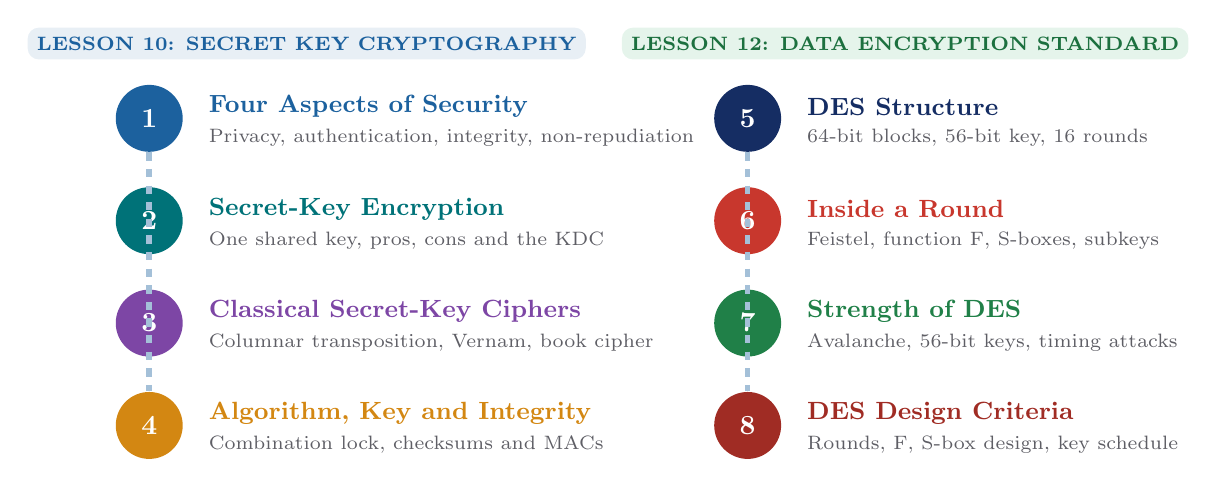
\begin{tikzpicture}
    \foreach \t/\c/\n [count=\i] in {
      Four Aspects of Security/ocean/Privacy\comma{} authentication\comma{} integrity\comma{} non-repudiation,
      Secret-Key Encryption/aqua!80!black/One shared key\comma{} pros\comma{} cons and the KDC,
      Classical Secret-Key Ciphers/grape/Columnar transposition\comma{} Vernam\comma{} book cipher,
      Algorithm\comma{} Key and Integrity/amber!90!black/Combination lock\comma{} checksums and MACs,
      DES Structure/navy/64-bit blocks\comma{} 56-bit key\comma{} 16 rounds,
      Inside a Round/brick/Feistel\comma{} function F\comma{} S-boxes\comma{} subkeys,
      Strength of DES/leaf!80!black/Avalanche\comma{} 56-bit keys\comma{} timing attacks,
      DES Design Criteria/brick!80!black/Rounds\comma{} F\comma{} S-box design\comma{} key schedule}
    {
      \pgfmathsetmacro{\x}{ifthenelse(\i<5,0,7.6)}
      \pgfmathsetmacro{\y}{-mod(\i-1,4)*1.3}
      \node[circle,fill=\c,text=white,font=\bfseries,minimum size=8.5mm] (n\i) at (\x,\y) {\i};
      \node[anchor=west,font=\small\bfseries,text=\c] at ([xshift=2mm,yshift=1.5mm]n\i.east) {\t};
      \node[anchor=west,font=\scriptsize,text=ink!75] at ([xshift=2mm,yshift=-2.5mm]n\i.east) {\n};
    }
    \draw[ocean!40,line width=2pt,dashed] (n1) -- (n4);
    \draw[ocean!40,line width=2pt,dashed] (n5) -- (n8);
    \node[fill=ocean!10,rounded corners,font=\scriptsize\bfseries,text=ocean] at (2.0,0.95) {LESSON 10: SECRET KEY CRYPTOGRAPHY};
    \node[fill=leaf!12,rounded corners,font=\scriptsize\bfseries,text=leaf!70!black] at (9.6,0.95) {LESSON 12: DATA ENCRYPTION STANDARD};
  \end{tikzpicture}
\end{frame}

% ============================================================
\setcounter{section}{9}
\section{Secret Key Cryptography}
% ============================================================

\begin{frame}{What Do Internet Users Expect?}
  \begin{columns}[c]
    \begin{column}{0.5\textwidth}
      \centering
      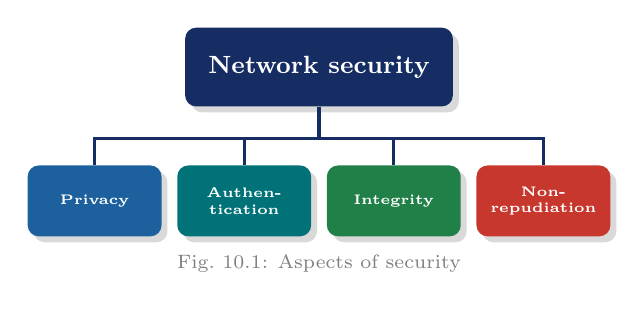
\begin{tikzpicture}
        \node[solid box=navy,minimum width=34mm,minimum height=10mm] (n) at (0,0) {Network security};
        \foreach \t/\c/\x [count=\i] in {Privacy/ocean/-2.85,Authen-\\tication/aqua!80!black/-0.95,Integrity/leaf!80!black/0.95,Non-\\repudiation/brick/2.85}{
          \node[solid box=\c,minimum width=17mm,minimum height=9mm,font=\tiny\bfseries] (a\i) at (\x,-1.7) {\t};
          \draw[navy,very thick] (n.south) -- ++(0,-0.4) -| (a\i.north);
        }
        \node[font=\scriptsize,text=ink!60] at (0,-2.5) {Fig.\ 10.1: Aspects of security};
      \end{tikzpicture}
    \end{column}
    \begin{column}{0.48\textwidth}
      {\small As more data travels over the Internet, users expect to:}
      \begin{itemize}\small\setlength{\itemsep}{3pt}
        \item keep messages \textbf{confidential}
        \item be sure of \textbf{data integrity}
        \item \textbf{identify} the sender of a message
        \item \textbf{prove} a message really came from a sender, even if the sender denies it
      \end{itemize}
      \begin{block}{So security has four aspects}
        \small Privacy, authentication, integrity and non-repudiation.
      \end{block}
    \end{column}
  \end{columns}
\end{frame}

% ------------------------------------------------------------
\begin{frame}{The Four Aspects Explained}
  \centering
  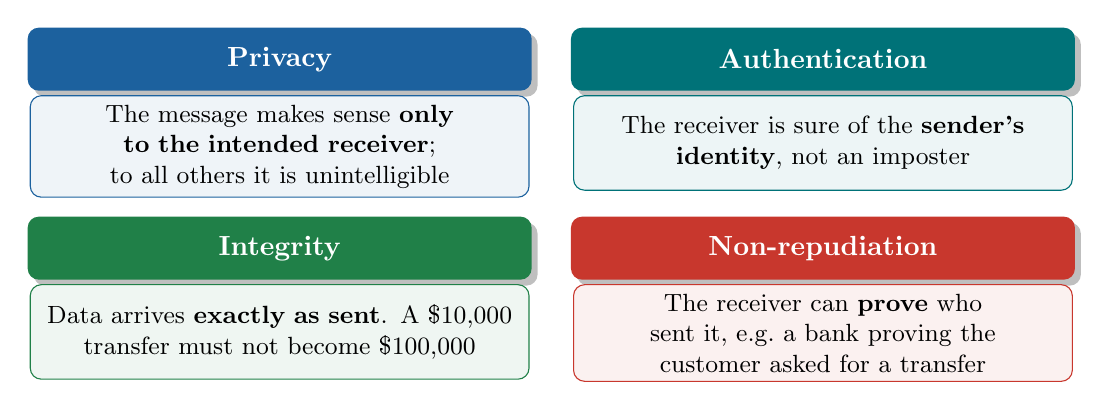
\begin{tikzpicture}
    \foreach \x/\y/\c/\t/\d in {
      0/0/ocean/Privacy/The message makes sense \textbf{only to the intended receiver}; to all others it is unintelligible,
      6.9/0/aqua!80!black/Authentication/The receiver is sure of the \textbf{sender's identity}\comma{} not an imposter,
      0/-2.4/leaf!80!black/Integrity/Data arrives \textbf{exactly as sent}. A \$10\comma{}000 transfer must not become \$100\comma{}000,
      6.9/-2.4/brick/Non-repudiation/The receiver can \textbf{prove} who sent it\comma{} e.g.\ a bank proving the customer asked for a transfer}
    {
      \node[fill=\c,text=white,rounded corners=4pt,font=\bfseries,minimum width=64mm,minimum height=8mm,drop shadow] (h) at (\x,\y) {\t};
      \node[draw=\c,fill=\c!7,rounded corners=4pt,text width=61mm,minimum height=12mm,font=\small,anchor=north,align=center] at ([yshift=-0.5mm]h.south) {\d};
    }
  \end{tikzpicture}
  \vspace{2mm}

  {\small The burden of proof for non-repudiation falls on the \textbf{receiver}.}
\end{frame}

% ------------------------------------------------------------
\begin{frame}{Privacy: Plaintext and Ciphertext}
  \centering
  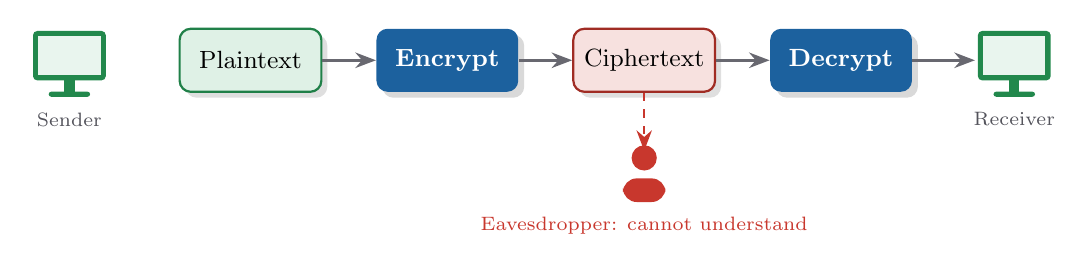
\begin{tikzpicture}
    \pic[scale=1.1] at (0,0) {pc=leaf}; \node[tag] at (0,-0.55) {Sender};
    \node[box=leaf,minimum width=18mm] (p) at (2.3,0.2) {Plaintext};
    \node[solid box=ocean,minimum width=18mm] (e) at (4.8,0.2) {Encrypt};
    \node[box=brick,minimum width=18mm] (c) at (7.3,0.2) {Ciphertext};
    \node[solid box=ocean,minimum width=18mm] (d) at (9.8,0.2) {Decrypt};
    \pic[scale=1.1] at (12,0) {pc=leaf}; \node[tag] at (12,-0.55) {Receiver};
    \draw[flow] (p) -- (e); \draw[flow] (e) -- (c); \draw[flow] (c) -- (d); \draw[flow] (d) -- (11.5,0.2);
    \pic at (7.3,-1.5) {person=brick}; \node[tag,text=brick] at (7.3,-1.9) {Eavesdropper: cannot understand};
    \draw[brick,dashed,thick,->] (c.south) -- (7.3,-0.95);
  \end{tikzpicture}
  \vspace{3mm}
  \begin{itemize}\small
    \item The concept of privacy \textbf{has not changed for thousands of years}: encrypt the message
    \item Data at the sender is \textbf{plaintext}; encrypted data is \textbf{ciphertext}, decrypted at the receiver
    \item Two categories of methods: \textbf{secret-key} methods and \textbf{public-key} methods
  \end{itemize}
\end{frame}

% ------------------------------------------------------------
\begin{frame}{Secret-Key Encryption (Fig.\ 10.2)}
  \centering
  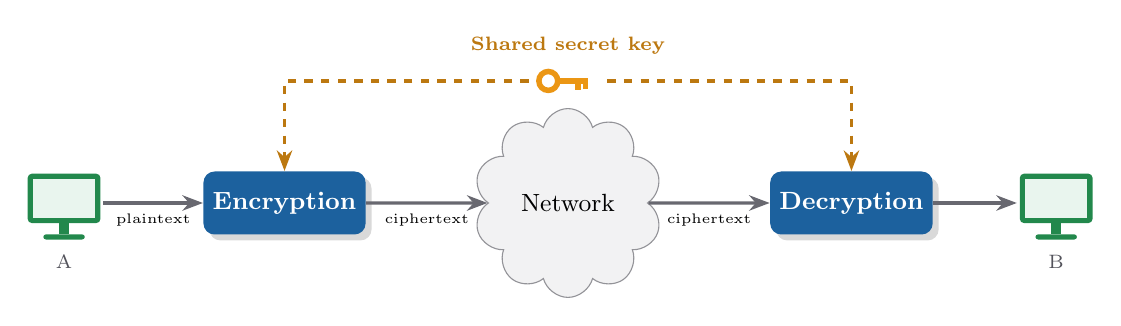
\begin{tikzpicture}
    \pic[scale=1.1] at (0,0) {pc=leaf}; \node[tag] at (0,-0.55) {A};
    \node[solid box=ocean,minimum width=20mm] (e) at (2.8,0.2) {Encryption};
    \node[cloud,cloud puffs=10,draw=ink!50,fill=ink!6,minimum width=2.4cm,minimum height=1.2cm,font=\small] (n) at (6.4,0.2) {Network};
    \node[solid box=ocean,minimum width=20mm] (d) at (10.0,0.2) {Decryption};
    \pic[scale=1.1] at (12.6,0) {pc=leaf}; \node[tag] at (12.6,-0.55) {B};
    \draw[flow] (0.5,0.2) -- node[below,font=\tiny]{plaintext} (e); \draw[flow] (e) -- node[below,font=\tiny]{ciphertext} (n);
    \draw[flow] (n) -- node[below,font=\tiny]{ciphertext} (d); \draw[flow] (d) -- (12.1,0.2);
    \pic at (6.15,1.75) {key=amber}; \node[font=\scriptsize\bfseries,text=amber!80!black] at (6.4,2.2) {Shared secret key};
    \draw[amber!80!black,dashed,very thick,->] (5.9,1.75) -| (e.north);
    \draw[amber!80!black,dashed,very thick,->] (6.9,1.75) -| (d.north);
  \end{tikzpicture}
  \vspace{3mm}
  \begin{columns}[T]
    \begin{column}{0.5\textwidth}
      \begin{block}{Key idea}
        \small The \textbf{same key} is used by the sender (to encrypt) and the receiver (to decrypt). The key is \textbf{shared}.
      \end{block}
    \end{column}
    \begin{column}{0.46\textwidth}
      \begin{itemize}\small
        \item Decryption is the \textbf{inverse} of encryption: if encryption adds and multiplies, decryption divides and subtracts
        \item Also called \textbf{symmetric} encryption: the same key works in both directions
      \end{itemize}
    \end{column}
  \end{columns}
\end{frame}

% ------------------------------------------------------------
\begin{frame}{Advantages and Disadvantages}
  \begin{columns}[T]
    \begin{column}{0.44\textwidth}
      \begin{exampleblock}{Advantage: efficiency}
        \small Secret-key algorithms take \textbf{less time} to encrypt than public-key ones, because the key is usually smaller. So they are used for \textbf{long messages}.
      \end{exampleblock}
      \begin{alertblock}{Disadvantages}
        \small
        1.~Each \textbf{pair} of users needs its own secret key\\
        2.~\textbf{Distributing} keys between parties can be difficult
      \end{alertblock}
    \end{column}
    \begin{column}{0.54\textwidth}
      \centering
      \begin{tikzpicture}
        \foreach \n/\r/\x in {3/0.75/0,4/0.75/2.2,5/0.75/4.4}{
          \foreach \i in {1,...,\n} \coordinate (p\i) at ($(\x,0)+(90+360/\n*\i:\r)$);
          \foreach \i in {1,...,\n} \foreach \j in {1,...,\n} {\ifnum\i<\j \draw[amber!80!black,thick] (p\i) -- (p\j);\fi}
          \foreach \i in {1,...,\n} \fill[ocean] (p\i) circle (0.11);
        }
        \node[font=\scriptsize] at (0,-1.1) {3 users: 3 keys};
        \node[font=\scriptsize] at (2.2,-1.1) {4 users: 6 keys};
        \node[font=\scriptsize] at (4.4,-1.1) {5 users: 10 keys};
        \node[fill=brick!12,draw=brick,rounded corners,font=\small,align=center] at (2.2,-2.2) {$N$ users need $\dfrac{N(N-1)}{2}$ keys\\[2pt]\scriptsize 1 million people $\Rightarrow$ about \textbf{500 billion} keys};
      \end{tikzpicture}
    \end{column}
  \end{columns}
\end{frame}

% ------------------------------------------------------------
\begin{frame}{Key Distribution Center (KDC)}
  \centering
  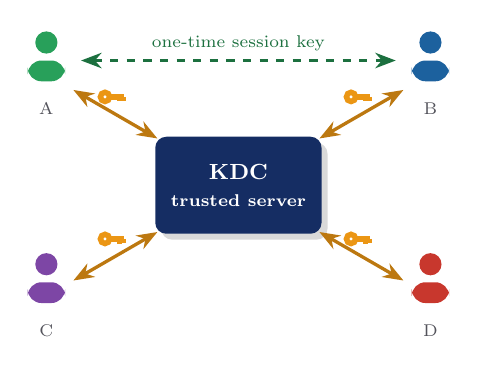
\begin{tikzpicture}[scale=0.88,transform shape]
    \node[solid box=navy,minimum width=24mm,minimum height=14mm] (k) at (0,0) {KDC\\\scriptsize trusted server};
    \foreach \a/\l/\c in {150/A/leaf,30/B/ocean,210/C/grape,330/D/brick}{
      \pic[scale=1] at (\a:3.2) {person=\c};
      \node[tag] at ($(\a:3.2)+(0,-0.5)$) {\l};
      \draw[amber!80!black,very thick,<->] ($(\a:2.75)$) -- ($(\a:1.35)$);
      \pic[scale=0.55] at ($(\a:2.05)+(-0.15,0.25)$) {key=amber};
    }
    \draw[leaf!70!black,very thick,dashed,<->] ($(150:3.2)+(0.5,0.2)$) -- node[above,font=\scriptsize]{one-time session key} ($(30:3.2)+(-0.5,0.2)$);
  \end{tikzpicture}
  \vspace{2mm}
  \begin{itemize}\small
    \item Two parties who may \textbf{never meet} must still agree on a shared secret key
    \item Solution: both \textbf{trust a third party}, the KDC, which shares one key with \textbf{each user}
    \item Users use their KDC key to set up a \textbf{one-time shared key} with each other
  \end{itemize}
  \begin{block}{Boxed rule}
    \small KDC can solve the problem of secret key distribution.
  \end{block}
\end{frame}

% ------------------------------------------------------------
\begin{frame}{Columnar Transposition: Round 1}
  \begin{columns}[c]
    \begin{column}{0.55\textwidth}
      \centering
      {\small Plaintext: \textbf{come home tomorrow}}\\[2mm]
      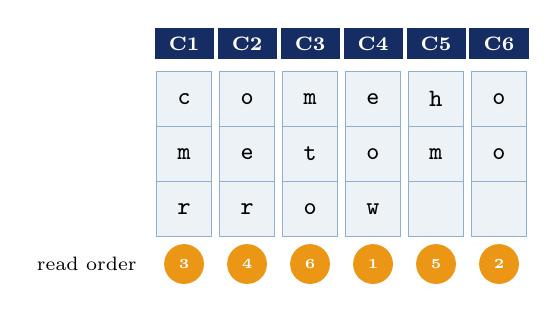
\begin{tikzpicture}[x=8mm,y=7mm]
        \foreach \c [count=\i] in {1,...,6} \node[fill=navy,text=white,font=\scriptsize\bfseries,minimum width=7.5mm] at (\i,0) {C\i};
        \foreach \r/\row in {1/{c,o,m,e,h,o},2/{m,e,t,o,m,o},3/{r,r,o,w,{},{}}}{
          \foreach \l [count=\i] in \row \node[draw=ocean!50,fill=ocean!8,minimum size=7mm,font=\small\ttfamily] at (\i,-\r) {\l};
        }
        \foreach \o [count=\i] in {4,6,1,2,5,3} \node[circle,fill=amber,text=white,font=\tiny\bfseries,minimum size=4.5mm] at (\o,-4.0) {\i};
        \node[font=\scriptsize,anchor=east] at (0.4,-4.0) {read order};
      \end{tikzpicture}
    \end{column}
    \begin{column}{0.43\textwidth}
      \begin{enumerate}\small\setlength{\itemsep}{3pt}
        \item Write the message \textbf{row by row} in a rectangle of 6 columns
        \item Choose a random column order, e.g.\ \textbf{4\,6\,1\,2\,5\,3}
        \item Read the text \textbf{column by column} in that order
      \end{enumerate}
      \vspace{2mm}
      \begin{block}{Ciphertext after round 1}
        \centering\ttfamily\small eow\,oo\,cmr\,oer\,hm\,mto
      \end{block}
    \end{column}
  \end{columns}
\end{frame}

% ------------------------------------------------------------
\begin{frame}{Columnar Transposition: Multiple Rounds (Fig.\ 10.3)}
  \begin{columns}[c]
    \begin{column}{0.55\textwidth}
      \centering
      {\small Round 2 input: \textbf{eowoocmroerhmmto}}\\[2mm]
      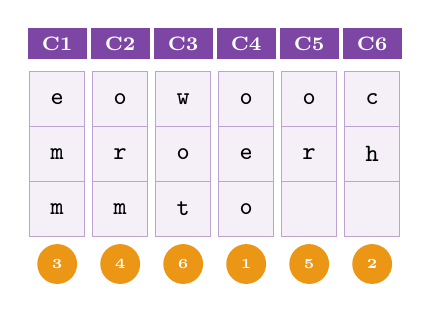
\begin{tikzpicture}[x=8mm,y=7mm]
        \foreach \c [count=\i] in {1,...,6} \node[fill=grape,text=white,font=\scriptsize\bfseries,minimum width=7.5mm] at (\i,0) {C\i};
        \foreach \r/\row in {1/{e,o,w,o,o,c},2/{m,r,o,e,r,h},3/{m,m,t,o,{},{}}}{
          \foreach \l [count=\i] in \row \node[draw=grape!50,fill=grape!8,minimum size=7mm,font=\small\ttfamily] at (\i,-\r) {\l};
        }
        \foreach \o [count=\i] in {4,6,1,2,5,3} \node[circle,fill=amber,text=white,font=\tiny\bfseries,minimum size=4.5mm] at (\o,-4.0) {\i};
      \end{tikzpicture}
    \end{column}
    \begin{column}{0.43\textwidth}
      \begin{enumerate}\small\setlength{\itemsep}{3pt}\setcounter{enumi}{3}
        \item Repeat steps 1--3 on the round-1 ciphertext
        \item Use the \textbf{same column order} 4\,6\,1\,2\,5\,3
        \item Continue for more rounds if desired
      \end{enumerate}
      \vspace{2mm}
      \begin{block}{Ciphertext after round 2}
        \centering\ttfamily\small oeo\,ch\,emm\,orm\,or\,wot
      \end{block}
      \begin{exampleblock}{Why repeat?}
        \small Multiple rounds make the ciphertext \textbf{much harder to crack} than one round.
      \end{exampleblock}
    \end{column}
  \end{columns}
\end{frame}

% ------------------------------------------------------------
\begin{frame}{Vernam Cipher (One-Time Pad)}
  \begin{columns}[c]
    \begin{column}{0.5\textwidth}
      \begin{block}{Idea}
        \small Use a \textbf{random, non-repeating} set of characters as the key (the pad). The pad is as long as the plaintext and is \textbf{never used again}, hence ``one-time''.
      \end{block}
      \begin{alertblock}{Algorithm (Fig.\ 10.4)}
        \small
        1.~Number letters: A=0, B=1, \dots, Z=25\\
        2.~Do the same for each pad letter\\
        3.~\textbf{Add} plaintext and pad numbers\\
        4.~If the sum $>25$, subtract 26\\
        5.~Turn the numbers back into letters
      \end{alertblock}
    \end{column}
    \begin{column}{0.48\textwidth}
      \centering
      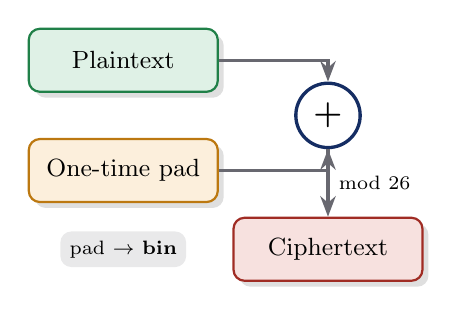
\begin{tikzpicture}
        \node[box=leaf,minimum width=24mm] (p) at (0,1.4) {Plaintext};
        \node[box=amber,minimum width=24mm] (k) at (0,0) {One-time pad};
        \node[circle,draw=navy,very thick,font=\large\bfseries,minimum size=8mm] (plus) at (2.6,0.7) {+};
        \node[box=brick,minimum width=24mm] (c) at (2.6,-1.0) {Ciphertext};
        \draw[flow] (p) -| (plus); \draw[flow] (k) -| (plus); \draw[flow] (plus) -- node[right,font=\scriptsize]{mod 26} (c);
        \node[fill=ink!10,rounded corners,font=\scriptsize] at (0,-1.0) {pad $\rightarrow$ \textbf{bin}};
      \end{tikzpicture}
    \end{column}
  \end{columns}
\end{frame}

% ------------------------------------------------------------
\begin{frame}{Vernam Cipher: Worked Example (Fig.\ 10.5)}
  \centering
  \renewcommand{\arraystretch}{1.25}
  \small
  \begin{tabular}{>{\bfseries}l *{9}{c}}
    \toprule
    \rowcolor{leaf!12} Plaintext & H & O & W & A & R & E & Y & O & U\\
    \rowcolor{leaf!12} & 7 & 14 & 22 & 0 & 17 & 4 & 24 & 14 & 20\\
    \rowcolor{amber!15} One-time pad & N & C & B & T & Z & Q & A & R & X\\
    \rowcolor{amber!15} & 13 & 2 & 1 & 19 & 25 & 16 & 0 & 17 & 23\\
    Sum & 20 & 16 & 23 & 19 & 42 & 20 & 24 & 31 & 43\\
    If $>25$, $-26$ & 20 & 16 & 23 & 19 & \textcolor{brick}{16} & 20 & 24 & \textcolor{brick}{5} & \textcolor{brick}{17}\\
    \rowcolor{brick!12} Ciphertext & U & Q & X & T & Q & U & Y & F & R\\
    \bottomrule
  \end{tabular}
  \vspace{3mm}
  \begin{columns}[T]
    \begin{column}{0.48\textwidth}
      \begin{exampleblock}{Strength}
        \small Pad discarded after one use, so it is \textbf{highly secure}. First built at \textbf{AT\&T} as the Vernam Machine.
      \end{exampleblock}
    \end{column}
    \begin{column}{0.48\textwidth}
      \begin{alertblock}{Weakness}
        \small A pad as long as the message, used once, is \textbf{impractical for large messages}. Suitable only for short ones.
      \end{alertblock}
    \end{column}
  \end{columns}
\end{frame}

% ------------------------------------------------------------
\begin{frame}{Book Cipher / Running Key Cipher}
  \begin{columns}[c]
    \begin{column}{0.48\textwidth}
      \centering
      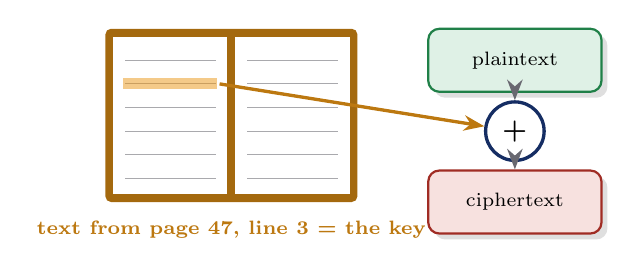
\begin{tikzpicture}
        \fill[amber!70!black,rounded corners=2pt] (-1.6,-1.1) rectangle (1.6,1.1);
        \fill[white] (-1.5,-1.0) rectangle (-0.05,1.0);
        \fill[white] (0.05,-1.0) rectangle (1.5,1.0);
        \foreach \y in {0.7,0.4,0.1,-0.2,-0.5,-0.8}{\draw[ink!40] (-1.35,\y) -- (-0.2,\y); \draw[ink!40] (0.2,\y) -- (1.35,\y);}
        \fill[amber,opacity=0.5] (-1.38,0.33) rectangle (-0.18,0.47);
        \node[font=\scriptsize\bfseries,text=amber!80!black] at (0,-1.45) {text from page 47, line 3 = the key};
        \node[box=leaf,minimum width=22mm,font=\scriptsize] (pt) at (3.6,0.7) {plaintext};
        \node[circle,draw=navy,very thick,font=\bfseries,minimum size=7mm] (pl) at (3.6,-0.2) {+};
        \node[box=brick,minimum width=22mm,font=\scriptsize] (ct) at (3.6,-1.1) {ciphertext};
        \draw[flow] (pt) -- (pl); \draw[flow] (pl) -- (ct); \draw[flow=amber!80!black] (-0.15,0.4) -- (pl);
      \end{tikzpicture}
    \end{column}
    \begin{column}{0.5\textwidth}
      \begin{itemize}\small\setlength{\itemsep}{4pt}
        \item Quite simple, and \textbf{similar in principle} to the Vernam cipher
        \item The ``pad'' is a portion of text from a \textbf{book}
        \item Book characters are \textbf{added} to the plaintext, just as with a one-time pad
      \end{itemize}
      \begin{block}{Practical advantage}
        \small Both parties only need to agree on a \textbf{book and a position}, instead of exchanging a long random pad.
      \end{block}
    \end{column}
  \end{columns}
\end{frame}

% ------------------------------------------------------------
\begin{frame}{Encryption and Decryption in the Real World (Fig.\ 10.8)}
  \centering
  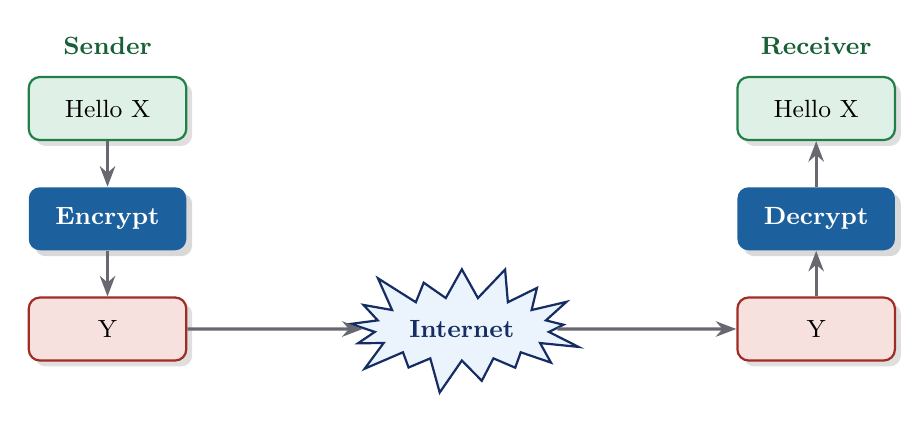
\begin{tikzpicture}
    \node[box=leaf,minimum width=20mm] (p1) at (0,1.4) {Hello X};
    \node[solid box=ocean,minimum width=20mm] (e) at (0,0) {Encrypt};
    \node[box=brick,minimum width=20mm] (c1) at (0,-1.4) {Y};
    \draw[flow] (p1) -- (e); \draw[flow] (e) -- (c1);
    \node[starburst,draw=navy,fill=sky,thick,minimum width=2.6cm,minimum height=1.8cm,font=\small\bfseries,text=navy] (net) at (4.5,-1.4) {Internet};
    \node[box=brick,minimum width=20mm] (c2) at (9,-1.4) {Y};
    \node[solid box=ocean,minimum width=20mm] (d) at (9,0) {Decrypt};
    \node[box=leaf,minimum width=20mm] (p2) at (9,1.4) {Hello X};
    \draw[flow] (c1) -- (net); \draw[flow] (net) -- (c2); \draw[flow] (c2) -- (d); \draw[flow] (d) -- (p2);
    \node[font=\small\bfseries,text=leaf!60!black] at (0,2.2) {Sender};
    \node[font=\small\bfseries,text=leaf!60!black] at (9,2.2) {Receiver};
  \end{tikzpicture}
  \vspace{3mm}
  \begin{columns}[T]
    \begin{column}{0.48\textwidth}
      \begin{block}{Encryption}
        \small Transforms \textbf{plaintext into ciphertext} at the sender's computer.
      \end{block}
    \end{column}
    \begin{column}{0.48\textwidth}
      \begin{block}{Decryption}
        \small The \textbf{exact opposite}: ciphertext back to plaintext at the receiver's computer.
      \end{block}
    \end{column}
  \end{columns}
\end{frame}

% ------------------------------------------------------------
\begin{frame}{Two Inputs: Algorithm and Key}
  \begin{columns}[c]
    \begin{column}{0.48\textwidth}
      \centering
      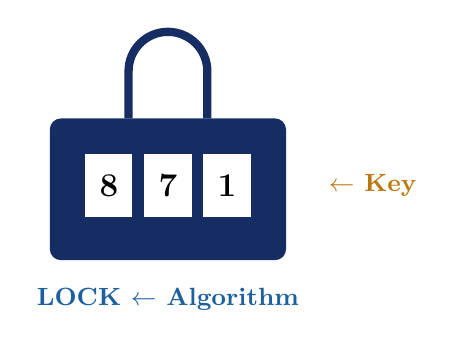
\begin{tikzpicture}
        \draw[navy,line width=3pt] (-0.5,0.9) -- (-0.5,1.5) arc (180:0:0.5) -- (0.5,0.9);
        \fill[navy,rounded corners=4pt] (-1.5,-0.9) rectangle (1.5,0.9);
        \foreach \x/\d in {-0.75/8,0/7,0.75/1} \node[fill=white,font=\large\bfseries,minimum width=6mm,minimum height=8mm] at (\x,0.05) {\d};
        \node[font=\small\bfseries,text=amber!80!black] at (2.6,0.05) {$\leftarrow$ Key};
        \node[font=\small\bfseries,text=ocean] at (0,-1.4) {LOCK $\leftarrow$ Algorithm};
      \end{tikzpicture}
    \end{column}
    \begin{column}{0.5\textwidth}
      \begin{itemize}\small\setlength{\itemsep}{3pt}
        \item The decryption algorithm must \textbf{match} the encryption algorithm, or the plaintext cannot be recovered
        \item The \textbf{key} is like the one-time pad: only sender and receiver know it
        \item A combination lock: everyone knows \textbf{how} it opens (algorithm), but only you know \textbf{871} (key)
      \end{itemize}
      \begin{alertblock}{The golden rule}
        \small The algorithm is usually \textbf{public}. It is the \textbf{secret key} that makes cryptography secure.
      \end{alertblock}
    \end{column}
  \end{columns}
\end{frame}

% ------------------------------------------------------------
\begin{frame}{Symmetric vs.\ Asymmetric Cryptography}
  \centering
  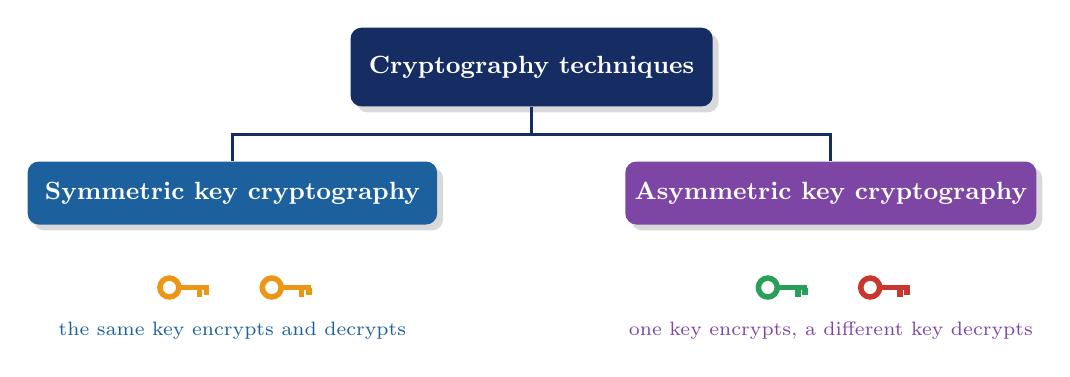
\begin{tikzpicture}
    \node[solid box=navy,minimum width=46mm,minimum height=10mm] (t) at (0,0) {Cryptography techniques};
    \node[solid box=ocean,minimum width=52mm] (s) at (-3.8,-1.6) {Symmetric key cryptography};
    \node[solid box=grape,minimum width=52mm] (a) at (3.8,-1.6) {Asymmetric key cryptography};
    \draw[navy,very thick] (t.south) -- ++(0,-0.35) -| (s.north);
    \draw[navy,very thick] (t.south) -- ++(0,-0.35) -| (a.north);
    \pic at (-4.6,-2.8) {key=amber}; \pic at (-3.3,-2.8) {key=amber};
    \node[font=\scriptsize,text=ocean] at (-3.8,-3.35) {the same key encrypts and decrypts};
    \pic at (3.0,-2.8) {key=leaf}; \pic at (4.3,-2.8) {key=brick};
    \node[font=\scriptsize,text=grape] at (3.8,-3.35) {one key encrypts, a different key decrypts};
  \end{tikzpicture}
  \vspace{3mm}
  \begin{block}{This module}
    \small Lesson 10 and DES are \textbf{symmetric}. Asymmetric (public-key) cryptography comes in \textbf{Module 8}.
  \end{block}
\end{frame}

% ------------------------------------------------------------
\begin{frame}{The Lock-and-Key Problem (Fig.\ 10.13)}
  \begin{columns}[c]
    \begin{column}{0.5\textwidth}
      \centering
      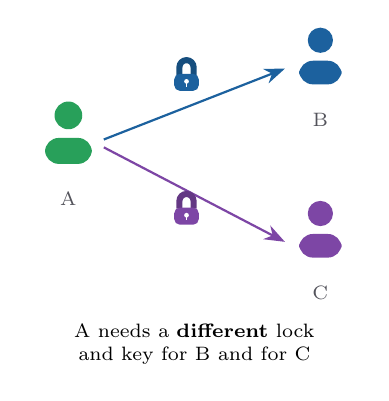
\begin{tikzpicture}
        \pic[scale=1.1] at (0,0) {person=leaf}; \node[tag] at (0,-0.55) {A};
        \pic[scale=1.0] at (3.2,1.0) {person=ocean}; \node[tag] at (3.2,0.45) {B};
        \pic[scale=1.0] at (3.2,-1.2) {person=grape}; \node[tag] at (3.2,-1.75) {C};
        \draw[->,ocean,thick] (0.45,0.2) -- (2.75,1.1); \draw[->,grape,thick] (0.45,0.1) -- (2.75,-1.1);
        \pic[scale=0.6] at (1.5,0.95) {lock=ocean}; \pic[scale=0.6] at (1.5,-0.75) {lock=grape};
        \node[font=\scriptsize,text width=40mm,align=center] at (1.6,-2.4) {A needs a \textbf{different} lock and key for B and for C};
      \end{tikzpicture}
    \end{column}
    \begin{column}{0.48\textwidth}
      \renewcommand{\arraystretch}{1.25}
      \small
      \begin{tabular}{l c}
        \toprule
        \rowcolor{navy}\textcolor{white}{\textbf{Parties}} & \textcolor{white}{\textbf{Lock-and-key pairs}}\\
        \midrule
        2 (A, B) & 1\\
        3 (A, B, C) & 3\\
        4 (A, B, C, D) & 6\\
        5 (A, B, C, D, E) & 10\\
        \bottomrule
      \end{tabular}\\[3mm]
      {\small If B and C had the same key, B could open C's box. So every pair needs its \textbf{own} key.}
    \end{column}
  \end{columns}
\end{frame}

% ------------------------------------------------------------
\begin{frame}{Integrity Check: From Checksum to MAC}
  \centering
  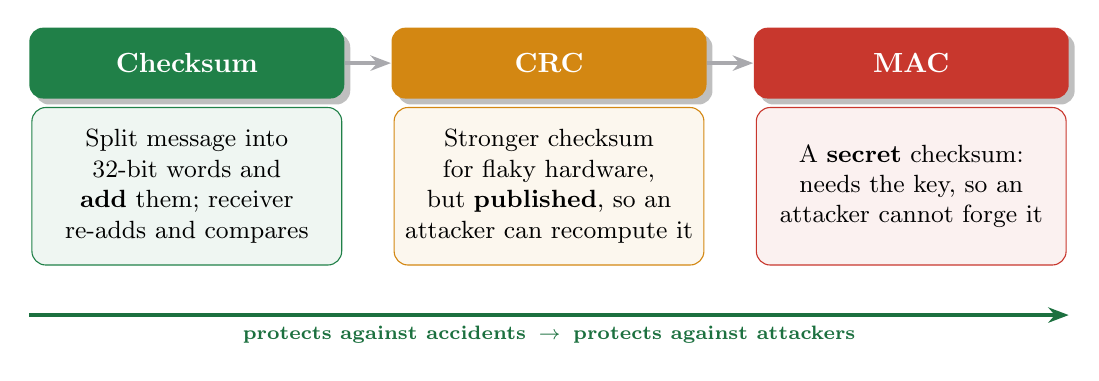
\begin{tikzpicture}
    \foreach \t/\c/\d [count=\i from 0] in {
      Checksum/leaf!80!black/Split message into 32-bit words and \textbf{add} them; receiver re-adds and compares,
      CRC/amber!90!black/Stronger checksum for flaky hardware\comma{} but \textbf{published}\comma{} so an attacker can recompute it,
      MAC/brick/A \textbf{secret} checksum: needs the key\comma{} so an attacker cannot forge it}
    {
      \node[fill=\c,text=white,rounded corners=5pt,font=\bfseries,minimum width=40mm,minimum height=9mm,drop shadow] (h\i) at (\i*4.6,0) {\t};
      \node[draw=\c,fill=\c!7,rounded corners=5pt,text width=37mm,minimum height=20mm,font=\small,anchor=north,align=center] at ([yshift=-1mm]h\i.south) {\d};
    }
    \draw[->,very thick,ink!40] (h0) -- (h1); \draw[->,very thick,ink!40] (h1) -- (h2);
    \draw[->,very thick,leaf!70!black] (-2,-3.2) -- node[below,font=\scriptsize\bfseries]{protects against accidents \,$\rightarrow$\, protects against attackers} (11.2,-3.2);
  \end{tikzpicture}
\end{frame}

% ------------------------------------------------------------
\begin{frame}{Message Authentication Code (MAC)}
  \centering
  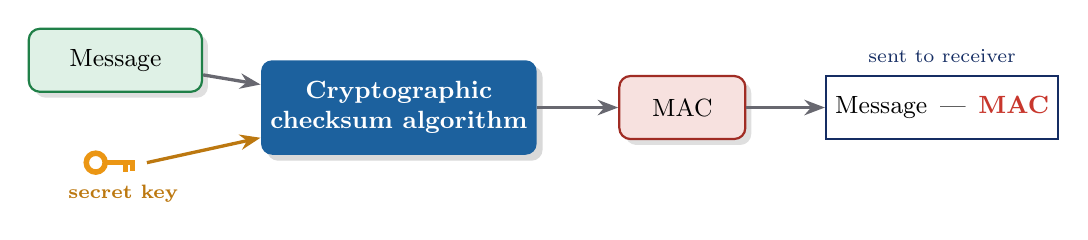
\begin{tikzpicture}
    \node[box=leaf,minimum width=22mm] (m) at (0,0.6) {Message};
    \pic at (-0.25,-0.7) {key=amber}; \node[font=\scriptsize\bfseries,text=amber!80!black] at (0.1,-1.1) {secret key};
    \node[solid box=ocean,minimum width=26mm,minimum height=12mm] (alg) at (3.6,0) {Cryptographic\\checksum algorithm};
    \node[box=brick,minimum width=16mm] (mac) at (7.2,0) {MAC};
    \draw[flow] (m) -- (alg); \draw[flow=amber!80!black] (0.4,-0.7) -- (alg);
    \draw[flow] (alg) -- (mac);
    \node[draw=navy,thick,fill=white,minimum height=8mm] (pk) at (10.5,0) {\small Message \,|\, \textcolor{brick}{\textbf{MAC}}};
    \draw[flow] (mac) -- (pk);
    \node[font=\scriptsize,text=navy] at (10.5,0.65) {sent to receiver};
  \end{tikzpicture}
  \vspace{3mm}
  \begin{columns}[T]
    \begin{column}{0.5\textwidth}
      \begin{itemize}\small\setlength{\itemsep}{2pt}
        \item As with encryption: a \textbf{known algorithm} plus a \textbf{secret key}
        \item Also called a \textbf{MIC} (message integrity code); MAC is the more popular term
        \item Used for years to protect large \textbf{interbank fund transfers}: not secret, but integrity is ensured
      \end{itemize}
    \end{column}
    \begin{column}{0.46\textwidth}
      \begin{alertblock}{How hard to forge?}
        \small A typical MAC is at least \textbf{48 bits}, so the chance of guessing it is about \textbf{1 in 280 trillion}.
      \end{alertblock}
    \end{column}
  \end{columns}
\end{frame}


% ------------------------------------------------------------
\begin{frame}{Quick Check: Lesson 10}
  \centering
  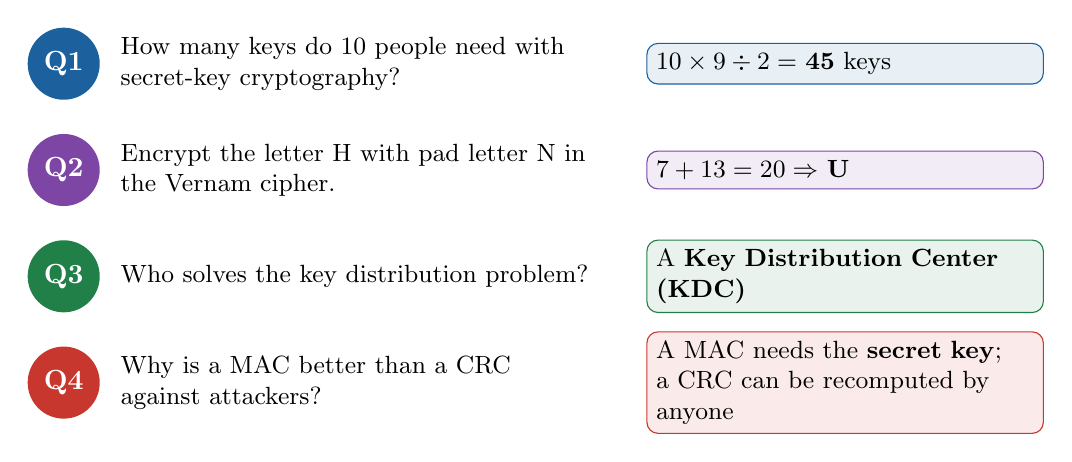
\begin{tikzpicture}
    \foreach \q/\a/\c [count=\i] in {
      How many keys do 10 people need with secret-key cryptography?/$10 \times 9 \div 2 = $ \textbf{45} keys/ocean,
      Encrypt the letter H with pad letter N in the Vernam cipher./$7 + 13 = 20 \Rightarrow$ \textbf{U}/grape,
      Who solves the key distribution problem?/A \textbf{Key Distribution Center (KDC)}/leaf!80!black,
      Why is a MAC better than a CRC against attackers?/A MAC needs the \textbf{secret key}; a CRC can be recomputed by anyone/brick}
    {
      \node[circle,fill=\c,text=white,font=\bfseries,minimum size=8mm] (n\i) at (0,-\i*1.35) {Q\i};
      \node[anchor=west,font=\small,text width=60mm] at (0.6,-\i*1.35) {\q};
      \node[anchor=west,fill=\c!10,draw=\c,rounded corners,font=\small,text width=48mm] at (7.4,-\i*1.35) {\a};
    }
  \end{tikzpicture}
\end{frame}

% ============================================================
\setcounter{section}{11}
\section{Data Encryption Standard}
% ============================================================

\begin{frame}{Confusion and Diffusion}
  \begin{columns}[T]
    \begin{column}{0.49\textwidth}
      \centering\textbf{\textcolor{ocean}{Substitution $\Rightarrow$ Confusion}}\\[2mm]
      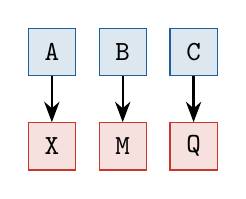
\begin{tikzpicture}
        \foreach \l [count=\i from 0] in {A,B,C} \node[fill=ocean!15,draw=ocean,font=\ttfamily,minimum size=6mm] (a\i) at (\i*0.9,0) {\l};
        \foreach \l [count=\i from 0] in {X,M,Q} {\node[fill=brick!15,draw=brick,font=\ttfamily,minimum size=6mm] (b\i) at (\i*0.9,-1.2) {\l}; \draw[->,thick] (a\i) -- (b\i);}
      \end{tikzpicture}\\[2mm]
      {\small A symbol is \textbf{replaced} by another. This hides the relationship between key and ciphertext.}
    \end{column}
    \begin{column}{0.49\textwidth}
      \centering\textbf{\textcolor{grape}{Transposition $\Rightarrow$ Diffusion}}\\[2mm]
      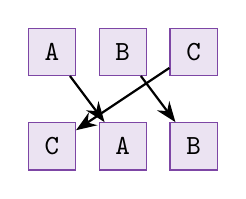
\begin{tikzpicture}
        \foreach \l [count=\i from 0] in {A,B,C} \node[fill=grape!15,draw=grape,font=\ttfamily,minimum size=6mm] (a\i) at (\i*0.9,0) {\l};
        \foreach \l/\s [count=\i from 0] in {C/2,A/0,B/1} {\node[fill=grape!15,draw=grape,font=\ttfamily,minimum size=6mm] (b\i) at (\i*0.9,-1.2) {\l}; \draw[->,thick] (a\s) -- (b\i);}
      \end{tikzpicture}\\[2mm]
      {\small The \textbf{order} is rearranged. This spreads each plaintext bit over many ciphertext bits.}
    \end{column}
  \end{columns}
  \vspace{3mm}
  \begin{block}{Product ciphers}
    \small Alternate substitution and transposition phases to get \textbf{both} confusion and diffusion. DES is such a product cipher.
  \end{block}
\end{frame}

% ------------------------------------------------------------
\begin{frame}{What Is DES?}
  \begin{columns}[c]
    \begin{column}{0.46\textwidth}
      \centering
      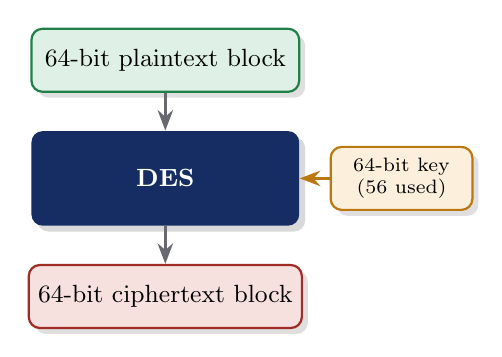
\begin{tikzpicture}
        \node[box=leaf,minimum width=34mm] (p) at (0,1.5) {64-bit plaintext block};
        \node[solid box=navy,minimum width=34mm,minimum height=12mm] (d) at (0,0) {DES};
        \node[box=brick,minimum width=34mm] (c) at (0,-1.5) {64-bit ciphertext block};
        \node[box=amber,minimum width=18mm,font=\scriptsize,align=center] (k) at (3.0,0) {64-bit key\\(56 used)};
        \draw[flow] (p) -- (d); \draw[flow] (d) -- (c); \draw[flow=amber!80!black] (k) -- (d);
      \end{tikzpicture}
    \end{column}
    \begin{column}{0.52\textwidth}
      \begin{itemize}\small\setlength{\itemsep}{3pt}
        \item Also called the \textbf{Data Encryption Algorithm (DEA)}
        \item Selected as an official US \textbf{FIPS} standard in \textbf{1976}; then used worldwide
        \item The archetypal \textbf{block cipher}: block size \textbf{64 bits}
        \item Key is 64 bits, but \textbf{8 are parity bits}, so the effective key is \textbf{56 bits}
        \item Intense study of DES shaped the modern understanding of block ciphers
      \end{itemize}
    \end{column}
  \end{columns}
\end{frame}

% ------------------------------------------------------------
\begin{frame}{Design Objectives of DES}
  \centering
  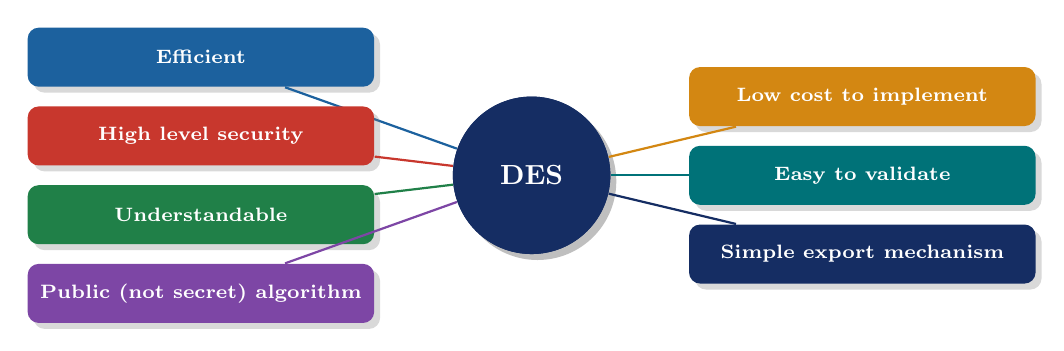
\begin{tikzpicture}
    \node[circle,fill=navy,text=white,font=\bfseries,minimum size=20mm,drop shadow] (c) at (0,0) {DES};
    \foreach \x/\y/\t/\c in {-4.2/1.5/Efficient/ocean,-4.2/0.5/High level security/brick,-4.2/-0.5/Understandable/leaf!80!black,-4.2/-1.5/Public (not secret) algorithm/grape,4.2/1.0/Low cost to implement/amber!90!black,4.2/0/Easy to validate/aqua!80!black,4.2/-1.0/Simple export mechanism/navy}{
      \node[solid box=\c,minimum width=44mm,minimum height=7.5mm,font=\scriptsize\bfseries] (s) at (\x,\y) {\t};
      \draw[\c,thick] (c) -- (s);
    }
    \node[circle,fill=navy,text=white,font=\bfseries,minimum size=20mm] at (0,0) {DES};
  \end{tikzpicture}
\end{frame}

% ------------------------------------------------------------
\begin{frame}{Overall Structure of DES (Fig.\ 12.1)}
  \begin{columns}[c]
    \begin{column}{0.56\textwidth}
      \centering
      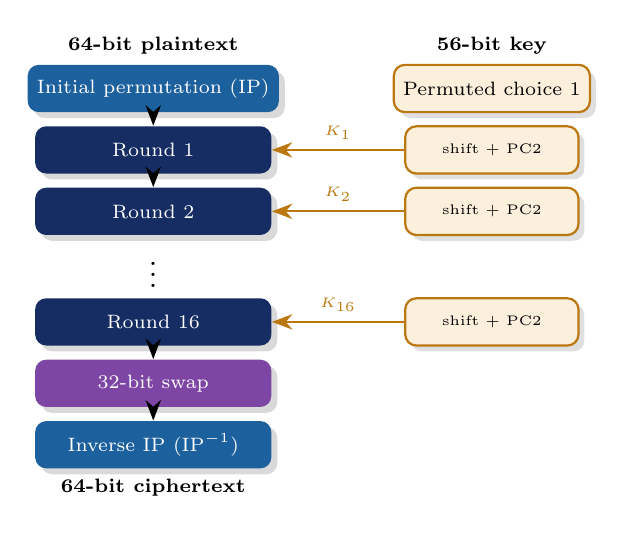
\begin{tikzpicture}[y=0.78cm]
        \node[font=\scriptsize\bfseries] at (0,0.7) {64-bit plaintext};
        \node[solid box=ocean,minimum width=30mm,minimum height=6mm,font=\scriptsize] (ip) at (0,0) {Initial permutation (IP)};
        \node[solid box=navy,minimum width=30mm,minimum height=6mm,font=\scriptsize] (r1) at (0,-1) {Round 1};
        \node[solid box=navy,minimum width=30mm,minimum height=6mm,font=\scriptsize] (r2) at (0,-2) {Round 2};
        \node[font=\large] at (0,-2.9) {$\vdots$};
        \node[solid box=navy,minimum width=30mm,minimum height=6mm,font=\scriptsize] (r16) at (0,-3.8) {Round 16};
        \node[solid box=grape,minimum width=30mm,minimum height=6mm,font=\scriptsize] (sw) at (0,-4.8) {32-bit swap};
        \node[solid box=ocean,minimum width=30mm,minimum height=6mm,font=\scriptsize] (fp) at (0,-5.8) {Inverse IP (IP$^{-1}$)};
        \node[font=\scriptsize\bfseries] at (0,-6.5) {64-bit ciphertext};
        \draw[->,thick] (ip) -- (r1); \draw[->,thick] (r1) -- (r2); \draw[->,thick] (r16) -- (sw); \draw[->,thick] (sw) -- (fp);
        \node[box=amber,minimum width=22mm,minimum height=6mm,font=\scriptsize] (pc1) at (4.3,0) {Permuted choice 1};
        \foreach \r/\y in {1/-1,2/-2,16/-3.8}{
          \node[box=amber,minimum width=22mm,minimum height=6mm,font=\tiny] (pc\r) at (4.3,\y) {shift + PC2};
          \draw[->,amber!80!black,thick] (pc\r.west) -- node[above,font=\tiny]{$K_{\r}$} (r\r.east);
        }
        \node[font=\scriptsize\bfseries] at (4.3,0.7) {56-bit key};
      \end{tikzpicture}
    \end{column}
    \begin{column}{0.42\textwidth}
      \begin{enumerate}\small\setlength{\itemsep}{3pt}
        \item \textbf{Initial permutation} rearranges the 64 plaintext bits
        \item \textbf{16 rounds} of the same function (permutation + substitution)
        \item Left and right halves are \textbf{swapped}
        \item \textbf{Inverse IP} produces the ciphertext
      \end{enumerate}
      \vspace{2mm}
      {\small On the right, the key passes through a permutation, then each round gets a \textbf{different subkey} $K_i$ from \textbf{left circular shifts} and a permutation.}
    \end{column}
  \end{columns}
\end{frame}

% ------------------------------------------------------------
\begin{frame}{One Round: The Feistel Structure}
  \begin{columns}[c]
    \begin{column}{0.5\textwidth}
      \centering
      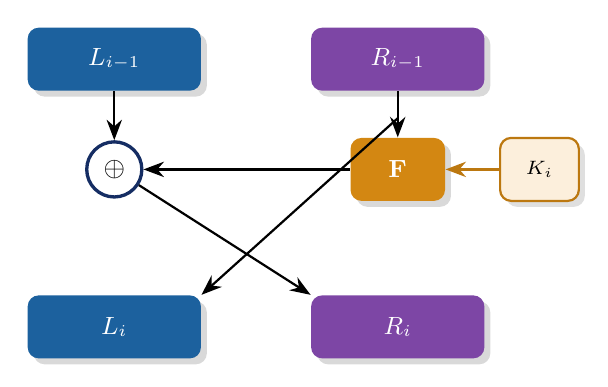
\begin{tikzpicture}
        \node[solid box=ocean,minimum width=22mm] (L0) at (0,0) {$L_{i-1}$};
        \node[solid box=grape,minimum width=22mm] (R0) at (3.6,0) {$R_{i-1}$};
        \node[solid box=amber!90!black,minimum width=12mm] (F) at (3.6,-1.4) {F};
        \node[circle,draw=navy,very thick,minimum size=7mm,font=\bfseries] (x) at (0,-1.4) {$\oplus$};
        \node[solid box=ocean,minimum width=22mm] (L1) at (0,-3.4) {$L_i$};
        \node[solid box=grape,minimum width=22mm] (R1) at (3.6,-3.4) {$R_i$};
        \draw[->,thick] (R0) -- (F);
        \node[box=amber,minimum width=10mm,font=\scriptsize] (k) at (5.4,-1.4) {$K_i$};
        \draw[->,thick,amber!80!black] (k) -- (F);
        \draw[->,thick] (F) -- (x); \draw[->,thick] (L0) -- (x);
        \draw[->,thick] (x) -- (R1.north west);
        \draw[->,thick] (3.6,-0.75) -- (L1.north east);
      \end{tikzpicture}
    \end{column}
    \begin{column}{0.48\textwidth}
      {\small Each 64-bit value is split into two 32-bit halves, \textbf{L} and \textbf{R}. Each round computes:}
      \begin{block}{Feistel formulas}
        \centering
        $L_i = R_{i-1}$\\[4pt]
        $R_i = L_{i-1} \oplus F(R_{i-1}, K_i)$
      \end{block}
      {\small $\oplus$ is bitwise XOR. Apart from the initial and final permutations, DES has \textbf{exactly the structure of a Feistel cipher}.}
    \end{column}
  \end{columns}
\end{frame}

% ------------------------------------------------------------
\begin{frame}{Inside the Function F (Fig.\ 12.3)}
  \begin{columns}[c]
    \begin{column}{0.56\textwidth}
      \centering
      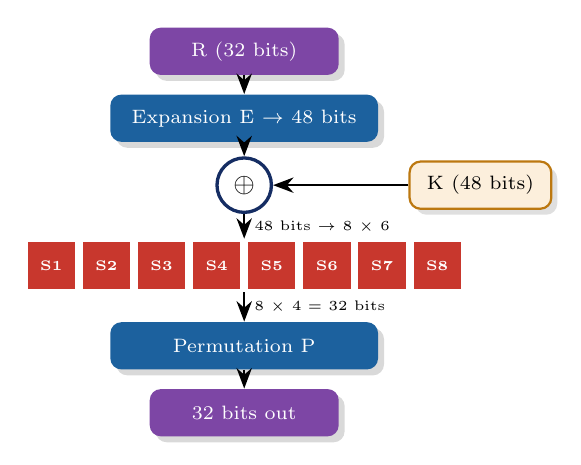
\begin{tikzpicture}[y=0.85cm]
        \node[solid box=grape,minimum width=24mm,minimum height=6mm,font=\scriptsize] (r) at (0,0) {R (32 bits)};
        \node[solid box=ocean,minimum width=34mm,minimum height=6mm,font=\scriptsize] (e) at (0,-1) {Expansion E $\rightarrow$ 48 bits};
        \node[circle,draw=navy,very thick,minimum size=6mm] (x) at (0,-2) {$\oplus$};
        \node[box=amber,minimum width=18mm,minimum height=6mm,font=\scriptsize] (k) at (3.0,-2) {K (48 bits)};
        \foreach \i in {1,...,8} \node[fill=brick,text=white,font=\tiny\bfseries,minimum width=6mm,minimum height=6mm] (s\i) at (-3.15+\i*0.7,-3.2) {S\i};
        \node[solid box=ocean,minimum width=34mm,minimum height=6mm,font=\scriptsize] (p) at (0,-4.4) {Permutation P};
        \node[solid box=grape,minimum width=24mm,minimum height=6mm,font=\scriptsize] (o) at (0,-5.4) {32 bits out};
        \draw[->,thick] (r) -- (e); \draw[->,thick] (e) -- (x); \draw[->,thick] (k) -- (x);
        \draw[->,thick] (x) -- node[right,font=\tiny]{48 bits $\rightarrow$ 8 $\times$ 6} (0,-2.8);
        \draw[->,thick] (0,-3.6) -- node[right,font=\tiny]{8 $\times$ 4 = 32 bits} (p); \draw[->,thick] (p) -- (o);
      \end{tikzpicture}
    \end{column}
    \begin{column}{0.42\textwidth}
      \begin{enumerate}\small\setlength{\itemsep}{3pt}
        \item The 32-bit R is \textbf{expanded} to 48 bits (16 bits duplicated)
        \item XORed with the 48-bit round key $K_i$
        \item Passed through \textbf{8 S-boxes}: each takes 6 bits and outputs 4
        \item The 32-bit result is \textbf{permuted} by P
      \end{enumerate}
      \begin{alertblock}{The S-boxes}
        \small The only \textbf{nonlinear} part of DES, and the heart of its security.
      \end{alertblock}
    \end{column}
  \end{columns}
\end{frame}

% ------------------------------------------------------------
\begin{frame}{How to Read an S-Box: Worked Example}
  \begin{columns}[c]
    \begin{column}{0.5\textwidth}
      \centering
      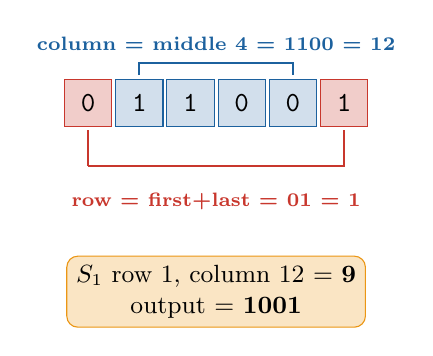
\begin{tikzpicture}[x=6.5mm]
        \foreach \b [count=\i from 0] in {0,1,1,0,0,1}{
          \pgfmathtruncatemacro{\edge}{(\i==0)||(\i==5)}
          \ifnum\edge=1 \node[fill=brick!25,draw=brick,font=\ttfamily\bfseries,minimum size=6mm] at (\i,0) {\b};
          \else \node[fill=ocean!20,draw=ocean,font=\ttfamily\bfseries,minimum size=6mm] at (\i,0) {\b}; \fi
        }
        \node[font=\scriptsize\bfseries,text=brick] at (2.5,-1.25) {row = first+last = 01 = 1};
        \node[font=\scriptsize\bfseries,text=ocean] at (2.5,0.75) {column = middle 4 = 1100 = 12};
        \draw[brick,thick] (0,-0.35) -- (0,-0.8) (5,-0.35) -- (5,-0.8) -- (0,-0.8);
        \draw[ocean,thick] (1,0.35) -- (1,0.5) -- (4,0.5) -- (4,0.35);
        \node[fill=amber!25,draw=amber,rounded corners,font=\small,align=center] at (2.5,-2.4) {$S_1$ row 1, column 12 = \textbf{9}\\output = \textbf{1001}};
      \end{tikzpicture}
    \end{column}
    \begin{column}{0.48\textwidth}
      \begin{itemize}\small\setlength{\itemsep}{4pt}
        \item Each S-box has \textbf{4 rows} and \textbf{16 columns}
        \item The \textbf{first and last} input bits pick the row (0--3)
        \item The \textbf{middle four} bits pick the column (0--15)
        \item The number in that cell, written in 4 bits, is the output
        \item Each row is a \textbf{reversible} substitution
      \end{itemize}
      \begin{block}{Example from the SLM}
        \small Input \texttt{011001} to $S_1$ gives output \texttt{1001}.
      \end{block}
    \end{column}
  \end{columns}
\end{frame}

% ------------------------------------------------------------
\begin{frame}{The Key Schedule}
  \centering
  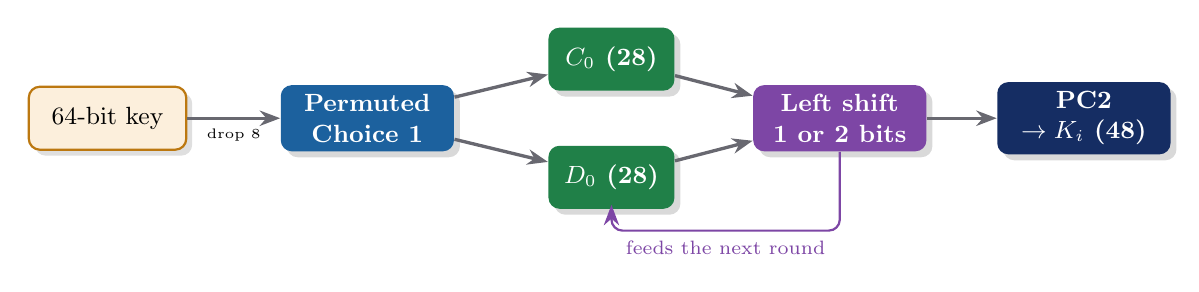
\begin{tikzpicture}
    \node[box=amber,minimum width=20mm] (k) at (0,0) {64-bit key};
    \node[solid box=ocean,minimum width=22mm,align=center] (pc1) at (3.3,0) {Permuted\\Choice 1};
    \node[solid box=leaf!80!black,minimum width=16mm] (c) at (6.4,0.75) {$C_0$ (28)};
    \node[solid box=leaf!80!black,minimum width=16mm] (d) at (6.4,-0.75) {$D_0$ (28)};
    \node[solid box=grape,minimum width=22mm,align=center] (sh) at (9.3,0) {Left shift\\1 or 2 bits};
    \node[solid box=navy,minimum width=22mm,align=center] (pc2) at (12.4,0) {PC2\\$\rightarrow K_i$ (48)};
    \draw[flow] (k) -- node[below,font=\tiny]{drop 8} (pc1); \draw[flow] (pc1) -- (c); \draw[flow] (pc1) -- (d);
    \draw[flow] (c) -- (sh); \draw[flow] (d) -- (sh); \draw[flow] (sh) -- (pc2);
    \draw[->,thick,grape,rounded corners] (sh.south) -- ++(0,-1.0) -| node[pos=0.25,below,font=\scriptsize]{feeds the next round} (6.4,-1.1);
\end{tikzpicture}
  \vspace{4mm}
  \begin{itemize}\small
    \item Bits are numbered 1--64; \textbf{every eighth bit is ignored}, leaving 56
    \item The 56 bits are split into two 28-bit halves, $C_0$ and $D_0$
    \item Each round, both halves rotate left by \textbf{1 or 2 bits}; Permuted Choice 2 then picks the \textbf{48-bit} subkey for $F(R_{i-1}, K_i)$
  \end{itemize}
\end{frame}

% ------------------------------------------------------------
\begin{frame}{DES Decryption and Characteristics}
  \begin{columns}[T]
    \begin{column}{0.48\textwidth}
      \begin{block}{Decryption}
        \small Same algorithm as encryption, with the subkeys in \textbf{reverse order}: $K_{16}$ first, then $K_{15}$, \dots, and $K_1$ last.
      \end{block}
      \centering
      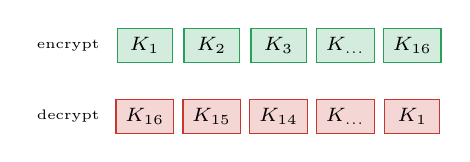
\begin{tikzpicture}
        \foreach \k [count=\i from 0] in {1,2,3,{\dots},16} \node[fill=leaf!20,draw=leaf,font=\scriptsize,minimum width=7mm] at (\i*0.85,0.6) {$K_{\k}$};
        \foreach \k [count=\i from 0] in {16,15,14,{\dots},1} \node[fill=brick!20,draw=brick,font=\scriptsize,minimum width=7mm] at (\i*0.85,-0.3) {$K_{\k}$};
        \node[font=\tiny,anchor=east] at (-0.45,0.6) {encrypt}; \node[font=\tiny,anchor=east] at (-0.45,-0.3) {decrypt};
      \end{tikzpicture}
    \end{column}
    \begin{column}{0.5\textwidth}
      \textbf{Characteristics of DES}
      \begin{enumerate}\small\setlength{\itemsep}{3pt}
        \item Each ciphertext bit depends on \textbf{all} key bits and \textbf{all} plaintext bits
        \item No \textbf{statistical relationship} between plaintext and ciphertext
        \item Changing one plaintext or key bit changes the ciphertext greatly (\textbf{avalanche effect})
        \item Changing ciphertext bits gives an \textbf{unpredictable} change in the recovered plaintext
      \end{enumerate}
    \end{column}
  \end{columns}
\end{frame}

% ------------------------------------------------------------
\begin{frame}{The Avalanche Effect (Table 12.1)}
  \begin{columns}[c]
    \begin{column}{0.56\textwidth}
      \centering
      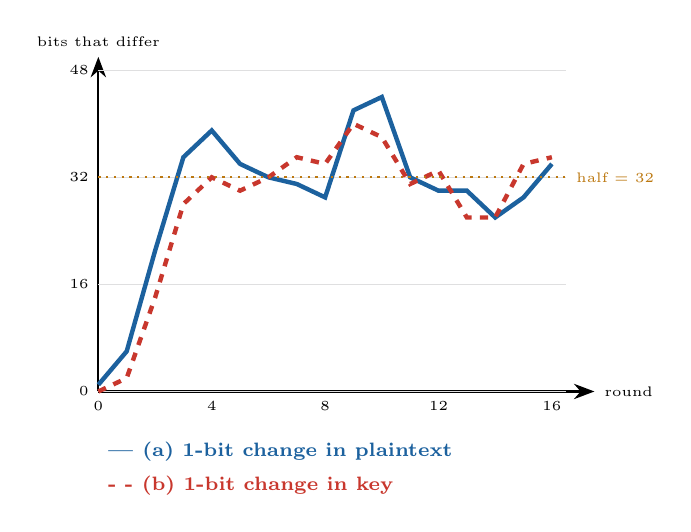
\begin{tikzpicture}[x=3.6mm,y=0.85mm]
        \draw[->,thick] (0,0) -- (17.5,0) node[right,font=\tiny]{round};
        \draw[->,thick] (0,0) -- (0,50) node[above,font=\tiny]{bits that differ};
        \foreach \y in {0,16,32,48} {\draw[ink!15] (0,\y) -- (16.5,\y); \node[font=\tiny,anchor=east] at (0,\y) {\y};}
        \foreach \x in {0,4,8,12,16} \node[font=\tiny,anchor=north] at (\x,0) {\x};
        \draw[ocean,line width=1.6pt] plot coordinates {(0,1)(1,6)(2,21)(3,35)(4,39)(5,34)(6,32)(7,31)(8,29)(9,42)(10,44)(11,32)(12,30)(13,30)(14,26)(15,29)(16,34)};
        \draw[brick,line width=1.6pt,dashed] plot coordinates {(0,0)(1,2)(2,14)(3,28)(4,32)(5,30)(6,32)(7,35)(8,34)(9,40)(10,38)(11,31)(12,33)(13,26)(14,26)(15,34)(16,35)};
        \draw[amber!80!black,thick,dotted] (0,32) -- (16.5,32) node[right,font=\tiny,text=amber!80!black]{half = 32};
        \node[font=\scriptsize\bfseries,text=ocean,anchor=west] at (0,-9) {\textbf{---} (a) 1-bit change in plaintext};
        \node[font=\scriptsize\bfseries,text=brick,anchor=west] at (0,-14) {\textbf{- -} (b) 1-bit change in key};
      \end{tikzpicture}
    \end{column}
    \begin{column}{0.42\textwidth}
      \begin{block}{Definition}
        \small A small change in the plaintext or the key should produce a \textbf{significant change} in the ciphertext.
      \end{block}
      \begin{itemize}\small\setlength{\itemsep}{3pt}
        \item Plaintexts differing by 1 bit: after \textbf{3 rounds}, 21 bits differ; at the end, \textbf{34}
        \item Keys differing by 1 bit: about \textbf{half} the ciphertext bits differ after a few rounds
      \end{itemize}
    \end{column}
  \end{columns}
\end{frame}

% ------------------------------------------------------------
\begin{frame}{Strength of DES: Three Kinds of Analysis}
  \centering
  \renewcommand{\arraystretch}{1.6}
  \begin{tabular}{>{\bfseries}l c l}
    \toprule
    \rowcolor{navy}\textcolor{white}{Type of analysis} & \textcolor{white}{\textbf{Order of search}} & \textcolor{white}{\textbf{Type of attack}}\\
    \midrule
    \textcolor{brick}{Exhaustive key search} & $O(2^{56})$ & Key attack\\
    \textcolor{grape}{Differential cryptanalysis} & $O(2^{47})$ & Chosen plaintext\\
    \textcolor{ocean}{Linear cryptanalysis} & $O(2^{43})$ & Known plaintext\\
    \bottomrule
  \end{tabular}
  \vspace{5mm}

  
\begin{tikzpicture}
    \node[fill=sky,rounded corners,text width=12cm,align=center,font=\small,inner sep=6pt]
      {DES strength has been analysed since \textbf{1975}. The main worry has always been the \textbf{key size}: can 56 bits really provide security?};
  \end{tikzpicture}
\end{frame}

% ------------------------------------------------------------
\begin{frame}{Exhaustive Search: How DES Fell}
  \centering
  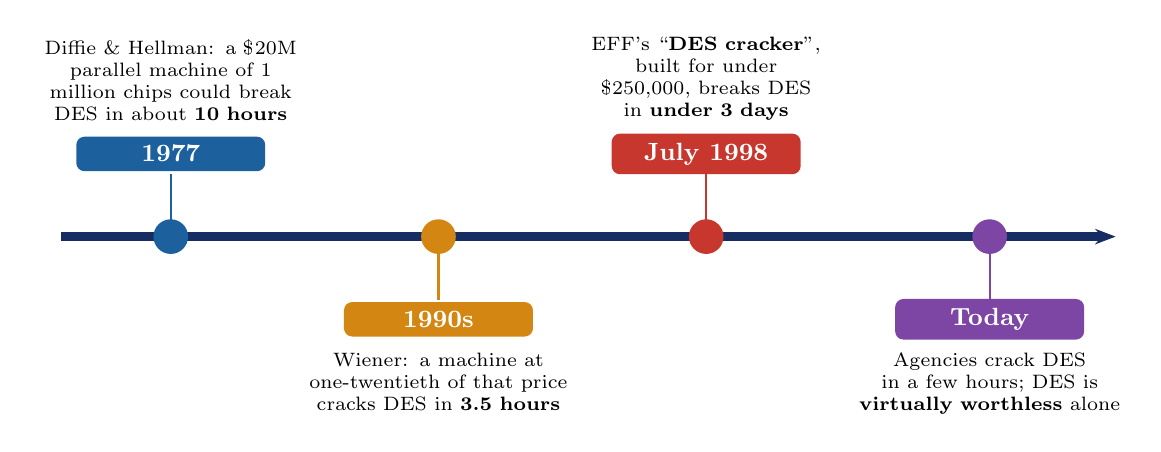
\begin{tikzpicture}
    \draw[navy,line width=3pt,->] (0,0) -- (13.4,0);
    \foreach \x/\c/\y/\t/\d in {
      1.4/ocean/1/1977/Diffie \& Hellman: a \$20M parallel machine of 1 million chips could break DES in about \textbf{10 hours},
      4.8/amber!90!black/-1/1990s/Wiener: a machine at one-twentieth of that price cracks DES in \textbf{3.5 hours},
      8.2/brick/1/July 1998/EFF's ``\textbf{DES cracker}''\comma{} built for under \$250\comma{}000\comma{} breaks DES in \textbf{under 3 days},
      11.8/grape/-1/Today/Agencies crack DES in a few hours; DES is \textbf{virtually worthless} alone}
    {
      \fill[\c] (\x,0) circle (2.2mm);
      \draw[\c,thick] (\x,0) -- (\x,\y*0.8);
      \node[fill=\c,text=white,rounded corners=3pt,font=\small\bfseries,minimum width=24mm] at (\x,\y*1.05) {\t};
      \ifnum\y>0 \node[font=\scriptsize,text width=34mm,align=center,anchor=south] at (\x,1.35) {\d};
      \else \node[font=\scriptsize,text width=34mm,align=center,anchor=north] at (\x,-1.35) {\d};\fi
    }
  \end{tikzpicture}
\end{frame}

% ------------------------------------------------------------
\begin{frame}{The Use of 56-Bit Keys}
  \begin{columns}[c]
    \begin{column}{0.48\textwidth}
      \centering
      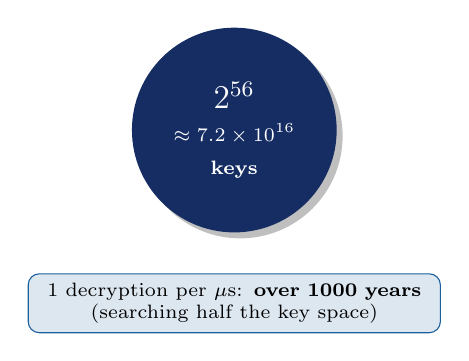
\begin{tikzpicture}
        \node[circle,fill=navy,text=white,font=\large\bfseries,minimum size=26mm,align=center,drop shadow] at (0,0) {$2^{56}$\\[-2pt]\scriptsize$\approx 7.2\times10^{16}$\\[-2pt]\scriptsize keys};
        \node[fill=ocean!15,draw=ocean,rounded corners,font=\scriptsize,text width=50mm,align=center] at (0,-2.2) {1 decryption per $\mu$s: \textbf{over 1000 years}\\(searching half the key space)};
      \end{tikzpicture}
    \end{column}
    \begin{column}{0.5\textwidth}
      \begin{itemize}\small\setlength{\itemsep}{4pt}
        \item At first sight, brute force on $2^{56}$ keys seems \textbf{impractical}
        \item But one decryption per microsecond is a very \textbf{conservative} assumption
        \item Hardware keeps getting cheaper and faster, as the EFF showed
      \end{itemize}
      \begin{alertblock}{It is more than trying keys}
        \small The attacker must \textbf{recognize} the correct plaintext. Easy for English text; harder if the data was \textbf{compressed} or is numerical.
      \end{alertblock}
    \end{column}
  \end{columns}
\end{frame}

% ------------------------------------------------------------
\begin{frame}{The Nature of the DES Algorithm}
  \begin{columns}[c]
    \begin{column}{0.45\textwidth}
      \centering
      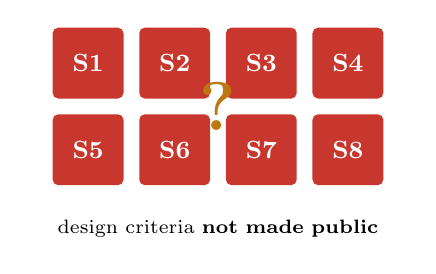
\begin{tikzpicture}
        \foreach \i in {1,...,8}{
          \pgfmathsetmacro{\x}{mod(\i-1,4)*1.1}
          \pgfmathsetmacro{\y}{-floor((\i-1)/4)*1.1}
          \node[fill=brick,text=white,font=\small\bfseries,minimum size=9mm,rounded corners=2pt] at (\x,\y) {S\i};
        }
        \node[font=\Huge\bfseries,text=amber!80!black] at (1.65,-0.55) {?};
        \node[font=\scriptsize,text width=46mm,align=center] at (1.65,-2.1) {design criteria \textbf{not made public}};
      \end{tikzpicture}
    \end{column}
    \begin{column}{0.53\textwidth}
      \begin{itemize}\small\setlength{\itemsep}{4pt}
        \item Concern: cryptanalysis may exploit the \textbf{characteristics of the algorithm}
        \item The focus is the \textbf{eight S-boxes} used in each iteration
        \item Since their design was secret, people suspected a hidden weakness known to an opponent
        \item Many regularities and odd behaviours have been found
      \end{itemize}
      \begin{exampleblock}{But\dots}
        \small No one has yet found the supposed \textbf{fatal weakness} in the S-boxes.
      \end{exampleblock}
    \end{column}
  \end{columns}
\end{frame}

% ------------------------------------------------------------
\begin{frame}{Timing Attacks}
  \begin{columns}[c]
    \begin{column}{0.48\textwidth}
      \centering
      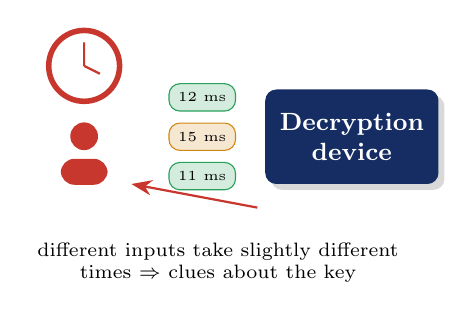
\begin{tikzpicture}
        \pic[scale=1.1] at (0,0) {person=brick};
        \draw[brick,line width=2pt,fill=white] (0,1.4) circle (0.45);
        \draw[brick,thick] (0,1.4) -- (0,1.7) (0,1.4) -- (0.2,1.3);
        \node[solid box=navy,minimum width=22mm,minimum height=12mm] (dev) at (3.4,0.5) {Decryption\\device};
        \foreach \t/\y/\c in {12 ms/1.0/leaf,15 ms/0.5/amber!90!black,11 ms/0.0/leaf}
          \node[fill=\c!20,draw=\c,font=\tiny,rounded corners] at (1.5,\y) {\t};
        \draw[->,thick,brick] (2.2,-0.4) -- (0.6,-0.1);
        \node[font=\scriptsize,text width=46mm,align=center] at (1.7,-1.1) {different inputs take slightly different times $\Rightarrow$ clues about the key};
      \end{tikzpicture}
    \end{column}
    \begin{column}{0.5\textwidth}
      \begin{block}{Definition}
        \small Information about the key or plaintext is found by \textbf{measuring how long} an implementation takes to decrypt different ciphertexts.
      \end{block}
      \begin{itemize}\small\setlength{\itemsep}{2pt}
        \item Attacks the \textbf{implementation}, not the algorithm
        \item Timing data is \textbf{easier to get} than mathematical flaws
        \item Defence: make every call take the \textbf{same time}, at the cost of slower response
        \item DES appears fairly resistant to timing attacks
      \end{itemize}
    \end{column}
  \end{columns}
\end{frame}

% ------------------------------------------------------------
\begin{frame}{DES Design Criteria: S-Boxes}
  \centering
  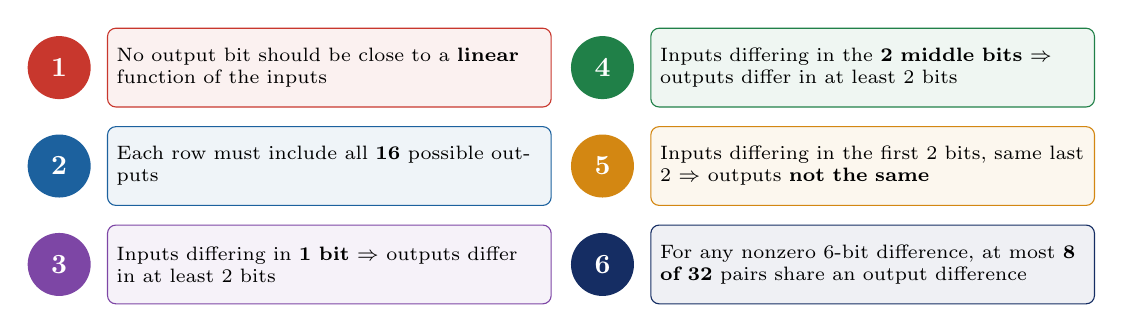
\begin{tikzpicture}
    \foreach \t/\c [count=\i] in {
      No output bit should be close to a \textbf{linear} function of the inputs/brick,
      Each row must include all \textbf{16} possible outputs/ocean,
      Inputs differing in \textbf{1 bit} $\Rightarrow$ outputs differ in at least 2 bits/grape,
      Inputs differing in the \textbf{2 middle bits} $\Rightarrow$ outputs differ in at least 2 bits/leaf!80!black,
      Inputs differing in the first 2 bits\comma{} same last 2 $\Rightarrow$ outputs \textbf{not the same}/amber!90!black,
      For any nonzero 6-bit difference\comma{} at most \textbf{8 of 32} pairs share an output difference/navy}
    {
      \pgfmathsetmacro{\x}{ifthenelse(\i<4,0,6.9)}
      \pgfmathsetmacro{\y}{-mod(\i-1,3)*1.25}
      \node[circle,fill=\c,text=white,font=\bfseries,minimum size=8mm] (c\i) at (\x,\y) {\i};
      \node[draw=\c,fill=\c!7,rounded corners=3pt,anchor=west,text width=54mm,minimum height=10mm,font=\scriptsize] at ([xshift=2mm]c\i.east) {\t};
    }
  \end{tikzpicture}
  \vspace{3mm}
  \begin{alertblock}{Why criterion 1 matters most}
    \small The S-boxes are the \textbf{only nonlinear} part of DES. If they were linear, the whole cipher would be linear and \textbf{easily broken} (like the Hill cipher).
  \end{alertblock}
\end{frame}

% ------------------------------------------------------------
\begin{frame}{DES Design Criteria: The Permutation P}
  \begin{columns}[c]
    \begin{column}{0.48\textwidth}
      \centering
      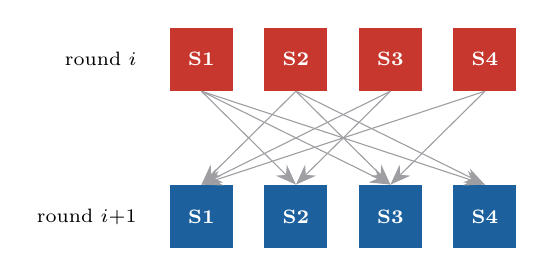
\begin{tikzpicture}
        \foreach \i in {1,...,4} \node[fill=brick,text=white,font=\scriptsize\bfseries,minimum size=8mm] (a\i) at (\i*1.2,1.5) {S\i};
        \foreach \i in {1,...,4} \node[fill=ocean,text=white,font=\scriptsize\bfseries,minimum size=8mm] (b\i) at (\i*1.2,-0.5) {S\i};
        \foreach \s/\t in {1/2,1/3,1/4,2/1,2/3,2/4,3/1,3/2,4/1,4/3}
          \draw[->,ink!45] (a\s.south) -- (b\t.north);
        \node[font=\scriptsize,anchor=east] at (0.5,1.5) {round $i$};
        \node[font=\scriptsize,anchor=east] at (0.5,-0.5) {round $i{+}1$};
      \end{tikzpicture}
    \end{column}
    \begin{column}{0.5\textwidth}
      \begin{enumerate}\small\setlength{\itemsep}{3pt}
        \item The 4 output bits of each S-box in round $i$: \textbf{two} feed ``middle bits'' and \textbf{two} feed ``end bits'' of round $i{+}1$
        \item The 4 outputs of each S-box affect \textbf{six different} S-boxes next round; no two affect the same one
        \item If an output of $S_j$ hits a middle bit of $S_k$, no output of $S_k$ may hit a middle bit of $S_j$
      \end{enumerate}
      \begin{block}{Goal}
        \small Increase the \textbf{diffusion} of the algorithm.
      \end{block}
    \end{column}
  \end{columns}
\end{frame}

% ------------------------------------------------------------
\begin{frame}{Number of Rounds and Function F}
  \begin{columns}[T]
    \begin{column}{0.49\textwidth}
      \centering
      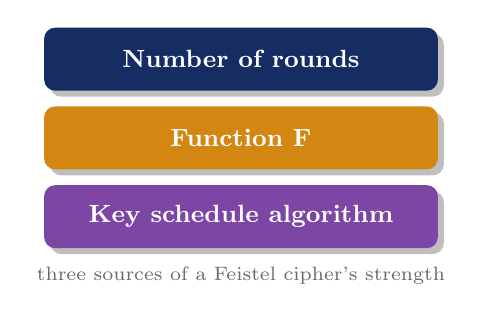
\begin{tikzpicture}
        \foreach \t/\c [count=\i from 0] in {Number of rounds/navy,Function F/amber!90!black,Key schedule algorithm/grape}
          \node[fill=\c,text=white,font=\small\bfseries,rounded corners=4pt,minimum width=50mm,minimum height=8mm,drop shadow] at (0,-\i*1.0) {\t};
        \node[font=\scriptsize,text=ink!70] at (0,-2.75) {three sources of a Feistel cipher's strength};
      \end{tikzpicture}
      \begin{block}{Rounds}
        \small More rounds make cryptanalysis harder, even with a weak F. Choose enough rounds that known attacks need \textbf{more effort than brute force}. DES followed this rule.
      \end{block}
    \end{column}
    \begin{column}{0.49\textwidth}
      \begin{alertblock}{Design of F}
        \small F is the \textbf{heart} of a Feistel cipher; in DES it relies on S-boxes. F provides \textbf{confusion}, so it must be hard to ``unscramble''.
      \end{alertblock}
      \begin{itemize}\small\setlength{\itemsep}{3pt}
        \item F must be \textbf{nonlinear}: the harder to approximate with linear equations, the better
        \item \textbf{Bit Independence Criterion (BIC):} output bits $j$ and $k$ change independently when any input bit $i$ flips
      \end{itemize}
    \end{column}
  \end{columns}
\end{frame}

% ------------------------------------------------------------
\begin{frame}{S-Box Design}
  \begin{columns}[c]
    \begin{column}{0.44\textwidth}
      \begin{itemize}\small\setlength{\itemsep}{3pt}
        \item Any input change should give a \textbf{random-looking} output change
        \item An $n \times m$ S-box has $n$ inputs and $m$ outputs; DES uses \textbf{6 $\times$ 4}
        \item Larger S-boxes resist cryptanalysis better, but the table grows \textbf{exponentially}; $n$ is usually limited to 8--10
      \end{itemize}
      \begin{exampleblock}{Key-dependent S-boxes}
        \small Random and key-based, so they cannot be analysed \textbf{in advance}.
      \end{exampleblock}
    \end{column}
    \begin{column}{0.54\textwidth}
      \centering\textbf{\textcolor{navy}{Nyberg's four approaches}}\\[2mm]
      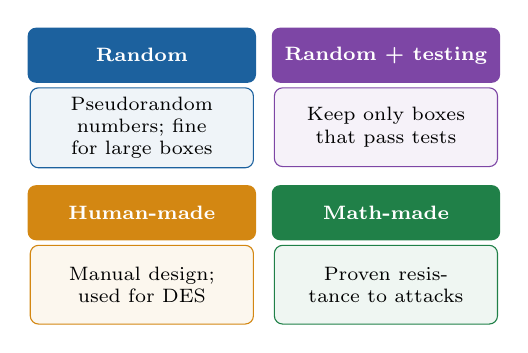
\begin{tikzpicture}
        \foreach \x/\y/\c/\t/\d in {
          0/0/ocean/Random/Pseudorandom numbers; fine for large boxes,
          3.1/0/grape/Random + testing/Keep only boxes that pass tests,
          0/-2.0/amber!90!black/Human-made/Manual design; used for DES,
          3.1/-2.0/leaf!80!black/Math-made/Proven resistance to attacks}
        {
          \node[fill=\c,text=white,font=\scriptsize\bfseries,rounded corners=3pt,minimum width=29mm,minimum height=7mm] (h) at (\x,\y) {\t};
          \node[draw=\c,fill=\c!7,rounded corners=3pt,text width=26mm,minimum height=10mm,font=\scriptsize,anchor=north,align=center] at ([yshift=-0.5mm]h.south) {\d};
        }
      \end{tikzpicture}
    \end{column}
  \end{columns}
\end{frame}

% ------------------------------------------------------------
\begin{frame}{Key Schedule Algorithm}
  \begin{columns}[c]
    \begin{column}{0.48\textwidth}
      \centering
      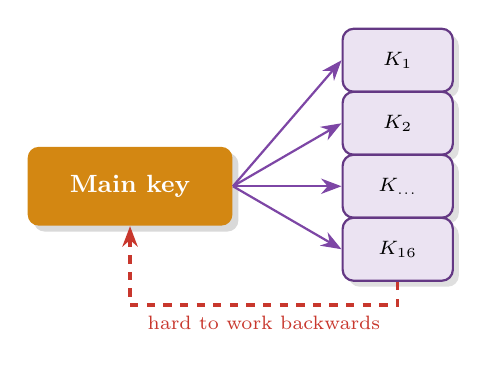
\begin{tikzpicture}
        \node[solid box=amber!90!black,minimum width=26mm,minimum height=10mm] (k) at (0,0) {Main key};
        \foreach \i/\y in {1/1.6,2/0.8,{\dots}/0,16/-0.8}{
          \node[box=grape,minimum width=14mm,font=\scriptsize] (s) at (3.4,\y) {$K_{\i}$};
          \draw[->,thick,grape] (k.east) -- (s.west);
        }
        \draw[<-,brick,very thick,dashed] (k.south) -- ++(0,-1.0) -| node[pos=0.25,below,font=\scriptsize,text=brick]{hard to work backwards} (3.4,-1.15);
      \end{tikzpicture}
    \end{column}
    \begin{column}{0.5\textwidth}
      \begin{itemize}\small\setlength{\itemsep}{4pt}
        \item Has received \textbf{less attention} than S-box design
        \item With any Feistel cipher, the key generates \textbf{one subkey per round}
        \item Subkeys should make it hard to \textbf{deduce individual subkeys}, and hard to work back to the \textbf{main key}
      \end{itemize}
      \begin{block}{Minimum requirement}
        \small Guarantee the \textbf{Strict Avalanche Criterion} and the \textbf{Bit Independence Criterion} for key/ciphertext.
      \end{block}
    \end{column}
  \end{columns}
\end{frame}

% ------------------------------------------------------------
\begin{frame}{DES at a Glance}
  \centering
  \renewcommand{\arraystretch}{1.45}
  \begin{tabular}{>{\bfseries}l l}
    \toprule
    \rowcolor{navy}\textcolor{white}{Feature} & \textcolor{white}{\textbf{DES}}\\
    \midrule
    Type & Symmetric block cipher (Feistel structure)\\
    Block size & 64 bits\\
    Key size & 64 bits, of which \textbf{56} are used (8 parity bits)\\
    Rounds & 16, each with its own 48-bit subkey\\
    Nonlinear part & 8 S-boxes, each $6 \rightarrow 4$ bits\\
    Decryption & Same algorithm, subkeys in reverse order\\
    Main weakness & Short key: broken by brute force (EFF, 1998)\\
    \bottomrule
  \end{tabular}
\end{frame}


% ------------------------------------------------------------
\begin{frame}{Quick Check: Lesson 12}
  \centering
  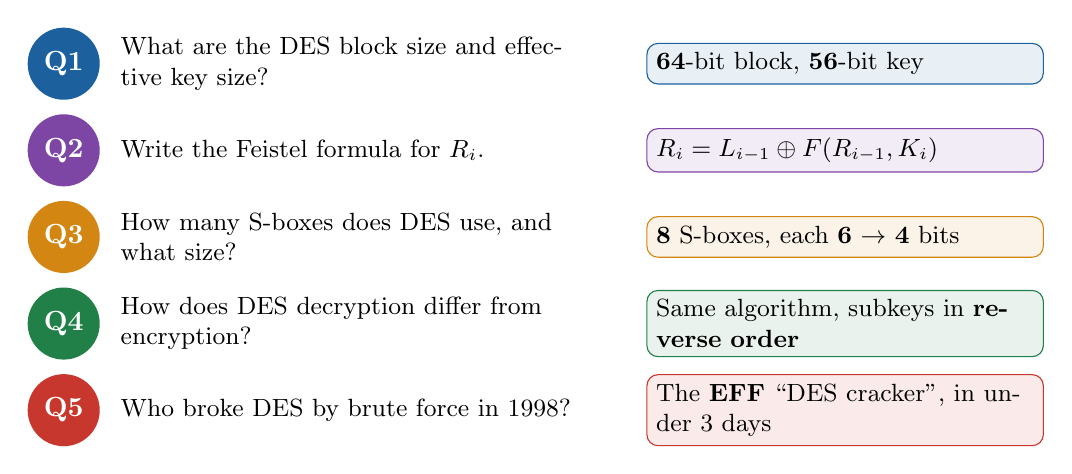
\begin{tikzpicture}
    \foreach \q/\a/\c [count=\i] in {
      What are the DES block size and effective key size?/\textbf{64}-bit block\comma{} \textbf{56}-bit key/ocean,
      Write the Feistel formula for $R_i$./$R_i = L_{i-1} \oplus F(R_{i-1}\comma{} K_i)$/grape,
      How many S-boxes does DES use\comma{} and what size?/\textbf{8} S-boxes\comma{} each \textbf{6 $\rightarrow$ 4} bits/amber!90!black,
      How does DES decryption differ from encryption?/Same algorithm\comma{} subkeys in \textbf{reverse order}/leaf!80!black,
      Who broke DES by brute force in 1998?/The \textbf{EFF} ``DES cracker''\comma{} in under 3 days/brick}
    {
      \node[circle,fill=\c,text=white,font=\bfseries,minimum size=8mm] (n\i) at (0,-\i*1.1) {Q\i};
      \node[anchor=west,font=\small,text width=60mm] at (0.6,-\i*1.1) {\q};
      \node[anchor=west,fill=\c!10,draw=\c,rounded corners,font=\small,text width=48mm] at (7.4,-\i*1.1) {\a};
    }
  \end{tikzpicture}
\end{frame}

% ------------------------------------------------------------
\begin{frame}{Module 6 Summary}
  \begin{columns}[T]
    \begin{column}{0.49\textwidth}
      \begin{block}{Lesson 10: Secret Key Cryptography}
        \small
        \begin{itemize}\setlength{\itemsep}{0pt}
          \item Privacy, authentication, integrity, non-repudiation
          \item One shared key; $N(N{-}1)/2$ keys; the KDC
          \item Columnar transposition with rounds
          \item Vernam (one-time pad) and book cipher
          \item Algorithm vs.\ key; symmetric vs.\ asymmetric
          \item Checksum, CRC and MAC
        \end{itemize}
      \end{block}
    \end{column}
    \begin{column}{0.49\textwidth}
      \begin{exampleblock}{Lesson 12: DES}
        \small
        \begin{itemize}\setlength{\itemsep}{0pt}
          \item Confusion, diffusion, product ciphers
          \item 64-bit block, 56-bit key, 16 Feistel rounds
          \item Function F, S-boxes, key schedule
          \item Avalanche effect; strength; timing attacks
          \item Design criteria for S-boxes, P, rounds, F
        \end{itemize}
      \end{exampleblock}
    \end{column}
  \end{columns}
  \vspace{1mm}
  \begin{alertblock}{Review questions}
    \scriptsize
    1.~Describe the features of secret key cryptography. \quad 2.~Explain methods of privacy implementation. \quad
    3.~Explain the Vernam cipher. \quad 4.~Discuss the book cipher. \quad 5.~Explain encryption and decryption in detail. \quad
    6.~Write a short note on integrity check. \quad 7.~Describe the overall structure of DES. \quad
    8.~Explain the avalanche effect in DES. \quad 9.~Discuss the DES design criteria.
  \end{alertblock}
\end{frame}

% ------------------------------------------------------------
\begin{frame}{References}
  \begin{enumerate}\setlength{\itemsep}{8pt}
    \item William Stallings, \emph{Cryptography and Network Security}, PHI Publishers.
    \item Charlie Kaufman, Radia Perlman, \emph{Network Security}, Pearson Education.
    \item Bruce Schneier, \emph{Applied Cryptography}, John Wiley \& Sons.
    \item Roberta Bragg, \emph{Network Security: The Complete Reference}, TMH.
  \end{enumerate}
  \vspace{6mm}
  \centering
  
\begin{tikzpicture}
    \node[fill=navy,text=white,rounded corners=8pt,inner sep=10pt,font=\Large\bfseries,drop shadow] {Thank You! \; Questions?};
  \end{tikzpicture}
\end{frame}

\end{document}
